% \documentclass[sigconf, authordraft]{acmart}
\documentclass[table, xcdraw, sigconf,review, anonymous]{acmart}
\acmConference[ESEC/FSE 2018]{12th Joint Meeting of the European Software Engineering Conference and the ACM SIGSOFT Symposium on the Foundations of Software Engineering}{4--9 November, 2018}{Lake Buena Vista, Florida}

\usepackage{booktabs} % For formal tables
\usepackage{url}

\usepackage{color}
\usepackage{enumitem}
\usepackage{xcolor}
\usepackage{listings}
\usepackage{graphicx} 
\usepackage{multirow}
\usepackage{siunitx}
\usepackage{rotating}
\usepackage{eqparbox}
\usepackage{wrapfig}
\usepackage{mathtools}
\usepackage{xspace}
\usepackage{enumitem}
\usepackage{hyperref}
\usepackage{lstlinebgrd}
\usepackage{amssymb}
\usepackage{amsmath}
\usepackage{hhline}

\usepackage{lstautogobble}
\usepackage[framemethod=tikz]{mdframed}
\usetikzlibrary{shadows}
\newmdenv[tikzsetting= {fill=white!20},roundcorner=10pt, shadow=true]{myshadowbox}
\usepackage{graphics}
\usepackage{colortbl} 
\usepackage{multirow} 
\usepackage{balance}
\usepackage{picture}
\usepackage{soul}
\usepackage{array}
\usepackage{makecell}


\usepackage{times}
\usepackage{wasysym}

\renewcommand\theadalign{cb}
\renewcommand\theadfont{\bfseries}
\renewcommand\theadgape{\Gape[4pt]}
\renewcommand\cellgape{\Gape[4pt]}

\newcommand\floor[1]{\lfloor#1\rfloor}
\newcommand\ceil[1]{\lceil#1\rceil}
\newcommand{\bibemph}[1]{{\em#1}}
\newcommand{\bibemphic}[1]{{\em#1\/}}
\newcommand{\bibsc}[1]{{\sc#1}}

\usepackage{verbatim}
\usepackage{algorithm}
\usepackage{algorithmicx}
\usepackage{algpseudocode}
\usepackage[export]{adjustbox}
\renewcommand{\footnotesize}{\scriptsize}
\usepackage{pgfplots}
\usepackage{pgfplotstable}
\pgfplotsset{compat=newest}
\usepackage{caption}


% Copyright
%\setcopyright{none}
%\setcopyright{acmcopyright}
%\setcopyright{acmlicensed}
\setcopyright{rightsretained}
%\setcopyright{usgov}
%\setcopyright{usgovmixed}
%\setcopyright{cagov}
%\setcopyright{cagovmixed}

\usepackage{verbatim}
\usepackage{algorithm}
\usepackage{algorithmicx}
\usepackage{algpseudocode}

\definecolor{MyDarkBlue}{rgb}{0,0.08,0.45} 
\lstset{
    language=Python,
    basicstyle=\sffamily\fontsize{2.3mm}{0.8em}\selectfont,
    breaklines=true,
    prebreak=\raisebox{0ex}[0ex][0ex]{\ensuremath{\hookleftarrow}},
    frame=l,
    showtabs=false,
    escapechar=|,
    columns=fullflexible,
    showspaces=false,
    showstringspaces=false,
    keywordstyle=\bfseries\sffamily,
    emph={generate, fitness, recombination_op, elitism, ML.train, model, find_best_model, model_building, this_dominates_that, normalize}, emphstyle=\bfseries\color{blue!50!black},
    stringstyle=\color{green!50!black},
    commentstyle=\color{red!50!black}\it,
    numbers=left,
    captionpos=t,
}


% DOI
\acmDOI{XX.YY/ZZ}

% ISBN
\acmISBN{ZZ-YY-24-ZZ/QQ/A}

%Conference
\acmConference[MSR'18]{Sweden}{May 2018}{} 
\acmYear{2018}
\copyrightyear{2018}

\acmPrice{15.00}

\acmSubmissionID{123-A12-B3}

\begin{document}
\title{
% Research and Teaching Tools for 
Resources for Data-Driven Search-Based SE}
% \titlenote{Produces the permission block, and
%   copyright information}
% \subtitle{Extended Abstract}
% \subtitlenote{The full version of the author's guide is available as
%   \texttt{acmart.pdf} document}

\author{Vivek Nair, George Mathew, Jianfeng Chen, Markus Wanger, Leando Minku, Tim Menzies}
\affiliation{%
  \institution{North Carolina State University, USA}
  \city{Raleigh} 
  \state{NC} 
  \postcode{27606}
}
\email{}


\begin{abstract}
This paper introduces tiny.cc/sbse, a  new shared resource for the Mining Software
Repositories (MSR) community.
The resource contains 89
artifacts related to data-driven search-based SE.
These artifacts are divided into 13 groups
such as requirements engineering, software product lines, software processes, etc.
Artifacts come with   meta-data about what papers have used 
the artifacts   in the past.   




This paper describes that resource,    how to use it,
and why the general MSR community might find it insightful.
The resource is a Github repository and our intent is that it
attracts enough attention that  other researchers  clone, modify, the submit  pull requests. In this way, we hope it grows
into a widely-used MSR resource.
\end{abstract}

%
% The code below should be generated by the tool at
% http://dl.acm.org/ccs.cfm
% Please copy and paste the code instead of the example below.
%
% \begin{CCSXML}
% <ccs2012>
%  <concept>
%   <concept_id>10010520.10010553.10010562</concept_id>
%   <concept_desc>Computer systems organization~Embedded systems</concept_desc>
%   <concept_significance>500</concept_significance>
%  </concept>
%  <concept>
%   <concept_id>10010520.10010575.10010755</concept_id>
%   <concept_desc>Computer systems organization~Redundancy</concept_desc>
%   <concept_significance>300</concept_significance>
%  </concept>
%  <concept>
%   <concept_id>10010520.10010553.10010554</concept_id>
%   <concept_desc>Computer systems organization~Robotics</concept_desc>
%   <concept_significance>100</concept_significance>
%  </concept>
%  <concept>
%   <concept_id>10003033.10003083.10003095</concept_id>
%   <concept_desc>Networks~Network reliability</concept_desc>
%   <concept_significance>100</concept_significance>
%  </concept>
% </ccs2012>
% \end{CCSXML}

% \ccsdesc[500]{Computer systems organization~Embedded systems}
% \ccsdesc[300]{Computer systems organization~Redundancy}
% \ccsdesc{Computer systems organization~Robotics}
% \ccsdesc[100]{Networks~Network reliability}


\keywords{}


\maketitle
\pagestyle{plain}
% \section{Introduction}

The \textit{proceedings} are the records of a conference.\footnote{This
  is a footnote}  ACM seeks
to give these conference by-products a uniform, high-quality
appearance.  To do this, ACM has some rigid requirements for the
format of the proceedings documents: there is a specified format
(balanced double columns), a specified set of fonts (Arial or
Helvetica and Times Roman) in certain specified sizes, a specified
live area, centered on the page, specified size of margins, specified
column width and gutter size.

\section{The Body of The Paper}
Typically, the body of a paper is organized into a hierarchical
structure, with numbered or unnumbered headings for sections,
subsections, sub-subsections, and even smaller sections.  The command
\texttt{{\char'134}section} that precedes this paragraph is part of
such a hierarchy.\footnote{This is a footnote.} \LaTeX\ handles the
numbering and placement of these headings for you, when you use the
appropriate heading commands around the titles of the headings.  If
you want a sub-subsection or smaller part to be unnumbered in your
output, simply append an asterisk to the command name.  Examples of
both numbered and unnumbered headings will appear throughout the
balance of this sample document.

Because the entire article is contained in the \textbf{document}
environment, you can indicate the start of a new paragraph with a
blank line in your input file; that is why this sentence forms a
separate paragraph.

\subsection{Type Changes and {\itshape Special} Characters}

We have already seen several typeface changes in this sample.  You can
indicate italicized words or phrases in your text with the command
\texttt{{\char'134}textit}; emboldening with the command
\texttt{{\char'134}textbf} and typewriter-style (for instance, for
computer code) with \texttt{{\char'134}texttt}.  But remember, you do
not have to indicate typestyle changes when such changes are part of
the \textit{structural} elements of your article; for instance, the
heading of this subsection will be in a sans serif\footnote{Another
  footnote here.  Let's make this a rather long one to see how it
  looks.} typeface, but that is handled by the document class file.
Take care with the use of\footnote{Another footnote.}  the
curly braces in typeface changes; they mark the beginning and end of
the text that is to be in the different typeface.

You can use whatever symbols, accented characters, or non-English
characters you need anywhere in your document; you can find a complete
list of what is available in the \textit{\LaTeX\ User's Guide}
\cite{Lamport:LaTeX}.

\subsection{Math Equations}
You may want to display math equations in three distinct styles:
inline, numbered or non-numbered display.  Each of
the three are discussed in the next sections.

\subsubsection{Inline (In-text) Equations}
A formula that appears in the running text is called an
inline or in-text formula.  It is produced by the
\textbf{math} environment, which can be
invoked with the usual \texttt{{\char'134}begin\,\ldots{\char'134}end}
construction or with the short form \texttt{\$\,\ldots\$}. You
can use any of the symbols and structures,
from $\alpha$ to $\omega$, available in
\LaTeX~\cite{Lamport:LaTeX}; this section will simply show a
few examples of in-text equations in context. Notice how
this equation:
\begin{math}
  \lim_{n\rightarrow \infty}x=0
\end{math},
set here in in-line math style, looks slightly different when
set in display style.  (See next section).

\subsubsection{Display Equations}
A numbered display equation---one set off by vertical space from the
text and centered horizontally---is produced by the \textbf{equation}
environment. An unnumbered display equation is produced by the
\textbf{displaymath} environment.

Again, in either environment, you can use any of the symbols
and structures available in \LaTeX\@; this section will just
give a couple of examples of display equations in context.
First, consider the equation, shown as an inline equation above:
\begin{equation}
  \lim_{n\rightarrow \infty}x=0
\end{equation}
Notice how it is formatted somewhat differently in
the \textbf{displaymath}
environment.  Now, we'll enter an unnumbered equation:
\begin{displaymath}
  \sum_{i=0}^{\infty} x + 1
\end{displaymath}
and follow it with another numbered equation:
\begin{equation}
  \sum_{i=0}^{\infty}x_i=\int_{0}^{\pi+2} f
\end{equation}
just to demonstrate \LaTeX's able handling of numbering.

\subsection{Citations}
Citations to articles~\cite{bowman:reasoning,
clark:pct, braams:babel, herlihy:methodology},
conference proceedings~\cite{clark:pct} or maybe
books \cite{Lamport:LaTeX, salas:calculus} listed
in the Bibliography section of your
article will occur throughout the text of your article.
You should use BibTeX to automatically produce this bibliography;
you simply need to insert one of several citation commands with
a key of the item cited in the proper location in
the \texttt{.tex} file~\cite{Lamport:LaTeX}.
The key is a short reference you invent to uniquely
identify each work; in this sample document, the key is
the first author's surname and a
word from the title.  This identifying key is included
with each item in the \texttt{.bib} file for your article.

The details of the construction of the \texttt{.bib} file
are beyond the scope of this sample document, but more
information can be found in the \textit{Author's Guide},
and exhaustive details in the \textit{\LaTeX\ User's
Guide} by Lamport~\shortcite{Lamport:LaTeX}.

This article shows only the plainest form
of the citation command, using \texttt{{\char'134}cite}.

Some examples.  A paginated journal article \cite{Abril07}, an enumerated
journal article \cite{Cohen07}, a reference to an entire issue \cite{JCohen96},
a monograph (whole book) \cite{Kosiur01}, a monograph/whole book in a series (see 2a in spec. document)
\cite{Harel79}, a divisible-book such as an anthology or compilation \cite{Editor00}
followed by the same example, however we only output the series if the volume number is given
\cite{Editor00a} (so Editor00a's series should NOT be present since it has no vol. no.),
a chapter in a divisible book \cite{Spector90}, a chapter in a divisible book
in a series \cite{Douglass98}, a multi-volume work as book \cite{Knuth97},
an article in a proceedings (of a conference, symposium, workshop for example)
(paginated proceedings article) \cite{Andler79}, a proceedings article
with all possible elements \cite{Smith10}, an example of an enumerated
proceedings article \cite{VanGundy07},
an informally published work \cite{Harel78}, a doctoral dissertation \cite{Clarkson85},
a master's thesis: \cite{anisi03}, an online document / world wide web
resource \cite{Thornburg01, Ablamowicz07, Poker06}, a video game (Case 1) \cite{Obama08} and (Case 2) \cite{Novak03}
and \cite{Lee05} and (Case 3) a patent \cite{JoeScientist001},
work accepted for publication \cite{rous08}, 'YYYYb'-test for prolific author
\cite{SaeediMEJ10} and \cite{SaeediJETC10}. Other cites might contain
'duplicate' DOI and URLs (some SIAM articles) \cite{Kirschmer:2010:AEI:1958016.1958018}.
Boris / Barbara Beeton: multi-volume works as books
\cite{MR781536} and \cite{MR781537}.

A couple of citations with DOIs: \cite{2004:ITE:1009386.1010128,
  Kirschmer:2010:AEI:1958016.1958018}.

Online citations: \cite{TUGInstmem, Thornburg01, CTANacmart}.


\subsection{Tables}
Because tables cannot be split across pages, the best
placement for them is typically the top of the page
nearest their initial cite.  To
ensure this proper ``floating'' placement of tables, use the
environment \textbf{table} to enclose the table's contents and
the table caption.  The contents of the table itself must go
in the \textbf{tabular} environment, to
be aligned properly in rows and columns, with the desired
horizontal and vertical rules.  Again, detailed instructions
on \textbf{tabular} material
are found in the \textit{\LaTeX\ User's Guide}.

Immediately following this sentence is the point at which
Table~\ref{tab:freq} is included in the input file; compare the
placement of the table here with the table in the printed
output of this document.

\begin{table}
  \caption{Frequency of Special Characters}
  \label{tab:freq}
  \begin{tabular}{ccl}
    \toprule
    Non-English or Math&Frequency&Comments\\
    \midrule
    \O & 1 in 1,000& For Swedish names\\
    $\pi$ & 1 in 5& Common in math\\
    \$ & 4 in 5 & Used in business\\
    $\Psi^2_1$ & 1 in 40,000& Unexplained usage\\
  \bottomrule
\end{tabular}
\end{table}

To set a wider table, which takes up the whole width of the page's
live area, use the environment \textbf{table*} to enclose the table's
contents and the table caption.  As with a single-column table, this
wide table will ``float'' to a location deemed more desirable.
Immediately following this sentence is the point at which
Table~\ref{tab:commands} is included in the input file; again, it is
instructive to compare the placement of the table here with the table
in the printed output of this document.


\begin{table*}
  \caption{Some Typical Commands}
  \label{tab:commands}
  \begin{tabular}{ccl}
    \toprule
    Command &A Number & Comments\\
    \midrule
    \texttt{{\char'134}author} & 100& Author \\
    \texttt{{\char'134}table}& 300 & For tables\\
    \texttt{{\char'134}table*}& 400& For wider tables\\
    \bottomrule
  \end{tabular}
\end{table*}
% end the environment with {table*}, NOTE not {table}!

It is strongly recommended to use the package booktabs~\cite{Fear05}
and follow its main principles of typography with respect to tables:
\begin{enumerate}
\item Never, ever use vertical rules.
\item Never use double rules.
\end{enumerate}
It is also a good idea not to overuse horizontal rules.


\subsection{Figures}

Like tables, figures cannot be split across pages; the best placement
for them is typically the top or the bottom of the page nearest their
initial cite.  To ensure this proper ``floating'' placement of
figures, use the environment \textbf{figure} to enclose the figure and
its caption.

This sample document contains examples of \texttt{.eps} files to be
displayable with \LaTeX.  If you work with pdf\LaTeX, use files in the
\texttt{.pdf} format.  Note that most modern \TeX\ systems will convert
\texttt{.eps} to \texttt{.pdf} for you on the fly.  More details on
each of these are found in the \textit{Author's Guide}.

\begin{figure}
\includegraphics{fly}
\caption{A sample black and white graphic.}
\end{figure}

\begin{figure}
\includegraphics[height=1in, width=1in]{fly}
\caption{A sample black and white graphic
that has been resized with the \texttt{includegraphics} command.}
\end{figure}


As was the case with tables, you may want a figure that spans two
columns.  To do this, and still to ensure proper ``floating''
placement of tables, use the environment \textbf{figure*} to enclose
the figure and its caption.  And don't forget to end the environment
with \textbf{figure*}, not \textbf{figure}!

\begin{figure*}
\includegraphics{flies}
\caption{A sample black and white graphic
that needs to span two columns of text.}
\end{figure*}


\begin{figure}
\includegraphics[height=1in, width=1in]{rosette}
\caption{A sample black and white graphic that has
been resized with the \texttt{includegraphics} command.}
\end{figure}

\subsection{Theorem-like Constructs}

Other common constructs that may occur in your article are the forms
for logical constructs like theorems, axioms, corollaries and proofs.
ACM uses two types of these constructs:  theorem-like and
definition-like.

Here is a theorem:
\begin{theorem}
  Let $f$ be continuous on $[a,b]$.  If $G$ is
  an antiderivative for $f$ on $[a,b]$, then
  \begin{displaymath}
    \int^b_af(t)\,dt = G(b) - G(a).
  \end{displaymath}
\end{theorem}

Here is a definition:
\begin{definition}
  If $z$ is irrational, then by $e^z$ we mean the
  unique number that has
  logarithm $z$:
  \begin{displaymath}
    \log e^z = z.
  \end{displaymath}
\end{definition}

The pre-defined theorem-like constructs are \textbf{theorem},
\textbf{conjecture}, \textbf{proposition}, \textbf{lemma} and
\textbf{corollary}.  The pre-defined de\-fi\-ni\-ti\-on-like constructs are
\textbf{example} and \textbf{definition}.  You can add your own
constructs using the \textsl{amsthm} interface~\cite{Amsthm15}.  The
styles used in the \verb|\theoremstyle| command are \textbf{acmplain}
and \textbf{acmdefinition}.

Another construct is \textbf{proof}, for example,

\begin{proof}
  Suppose on the contrary there exists a real number $L$ such that
  \begin{displaymath}
    \lim_{x\rightarrow\infty} \frac{f(x)}{g(x)} = L.
  \end{displaymath}
  Then
  \begin{displaymath}
    l=\lim_{x\rightarrow c} f(x)
    = \lim_{x\rightarrow c}
    \left[ g{x} \cdot \frac{f(x)}{g(x)} \right ]
    = \lim_{x\rightarrow c} g(x) \cdot \lim_{x\rightarrow c}
    \frac{f(x)}{g(x)} = 0\cdot L = 0,
  \end{displaymath}
  which contradicts our assumption that $l\neq 0$.
\end{proof}

\section{Conclusions}
This paragraph will end the body of this sample document.
Remember that you might still have Acknowledgments or
Appendices; brief samples of these
follow.  There is still the Bibliography to deal with; and
we will make a disclaimer about that here: with the exception
of the reference to the \LaTeX\ book, the citations in
this paper are to articles which have nothing to
do with the present subject and are used as
examples only.
%\end{document}  % This is where a 'short' article might terminate



\appendix
%Appendix A
\section{Headings in Appendices}
The rules about hierarchical headings discussed above for
the body of the article are different in the appendices.
In the \textbf{appendix} environment, the command
\textbf{section} is used to
indicate the start of each Appendix, with alphabetic order
designation (i.e., the first is A, the second B, etc.) and
a title (if you include one).  So, if you need
hierarchical structure
\textit{within} an Appendix, start with \textbf{subsection} as the
highest level. Here is an outline of the body of this
document in Appendix-appropriate form:
\subsection{Introduction}
\subsection{The Body of the Paper}
\subsubsection{Type Changes and  Special Characters}
\subsubsection{Math Equations}
\paragraph{Inline (In-text) Equations}
\paragraph{Display Equations}
\subsubsection{Citations}
\subsubsection{Tables}
\subsubsection{Figures}
\subsubsection{Theorem-like Constructs}
\subsubsection*{A Caveat for the \TeX\ Expert}
\subsection{Conclusions}
\subsection{References}
Generated by bibtex from your \texttt{.bib} file.  Run latex,
then bibtex, then latex twice (to resolve references)
to create the \texttt{.bbl} file.  Insert that \texttt{.bbl}
file into the \texttt{.tex} source file and comment out
the command \texttt{{\char'134}thebibliography}.
% This next section command marks the start of
% Appendix B, and does not continue the present hierarchy
\section{More Help for the Hardy}

Of course, reading the source code is always useful.  The file
\path{acmart.pdf} contains both the user guide and the commented
code.

\begin{acks}
  The authors would like to thank Dr. Yuhua Li for providing the
  MATLAB code of the \textit{BEPS} method.

  The authors would also like to thank the anonymous referees for
  their valuable comments and helpful suggestions. The work is
  supported by the \grantsponsor{GS501100001809}{National Natural
    Science Foundation of
    China}{http://dx.doi.org/10.13039/501100001809} under Grant
  No.:~\grantnum{GS501100001809}{61273304}
  and~\grantnum[http://www.nnsf.cn/youngscientists]{GS501100001809}{Young
    Scientists' Support Program}.

\end{acks}




\begin{figure*}[!t]
{\center
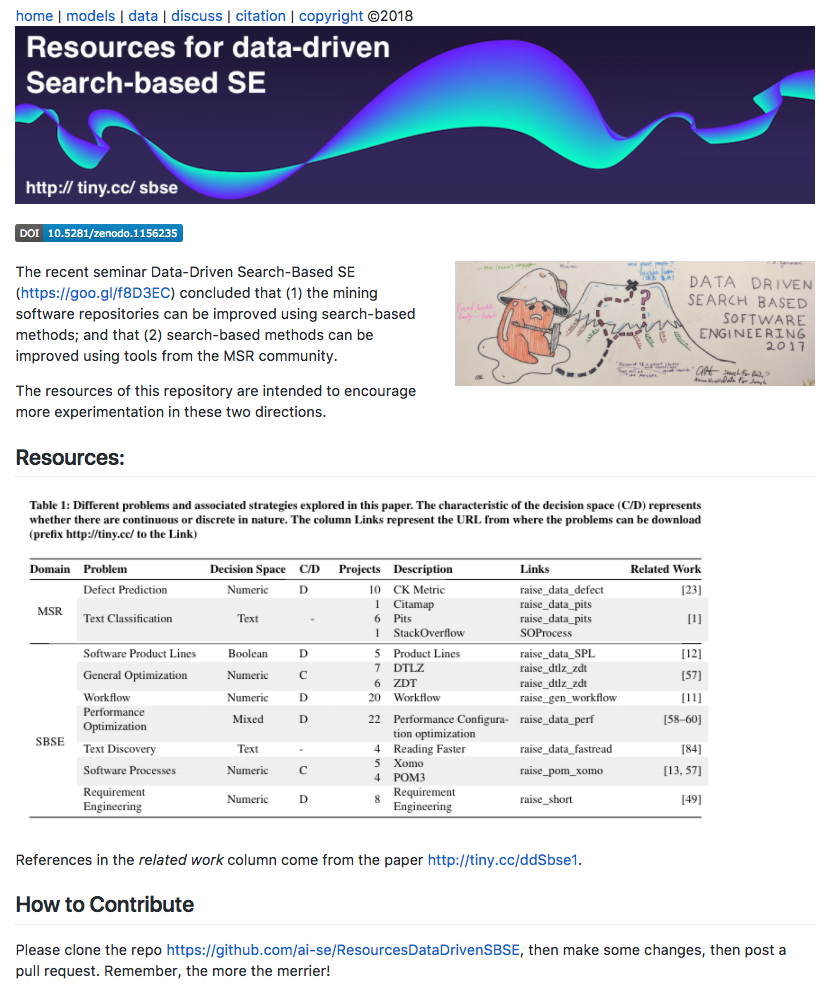
\includegraphics[width=5.5in]{img/page1.png}}
\caption{Our Github-based repository  for resources relating to data-driven Search-based SE.
http://tiny.cc/sbse}\label{fig:one}
\end{figure*}

\section{Introduction}


The MSR  community has benefited enormously from widely shared data sets.  Such data sets document the canonical problems in a field.
They serve to cluster together like-minded researchers while  
  allowing   them to generate reproducible results. Also, such data can be used by
   newcomers to learn state-of-the-set methods in this field. Further, they enable the mainstay of good science:
reputable, repeatable,  improvable, and even refutable results.
At the time of this writing,   nine of the 50 most cited papers in the last 5 years at IEEE Transactions of Software Engineering all draw their case studies
from a small number of similar defect prediction data sets.


As a field evolves, so too should its canonical problems. One  reason for the emergence of   MSR  in 2004 was the existence of a new generation of widely-available data mining
algorithms that could scale to interestingly large problems.  Now, some 14 years later, a new technology has emerged that could reshape the future of this community. There now exists numerous, readily
available, {\em search-based software engineering} (SBSE) algorithms. Whereas:
\begin{itemize}
\item
An MSR researcher might deploy a
data miner to learn a model from  dat   that predicts for (say) a single target class;
\item
An SBSE researcher might deploy a multi-objective optimizer
to find what examples score best
on multiple target variables.
\end{itemize}

There has been a recent increased in methods that combine MSR and SBSE.
A recent workshop  on {\em Data-drive Search-based Software
Engineering} (goo.gl/f8D3EC)   was well attended by over two dozen senior members of the MSR community.
The workshop concluded that (1) the mining software repositories can be improved using search-based methods; and that (2) search-based methods can be improved using tools from the MSR community. 
For example:
\begin{itemize}
\item
MSR data mining algorithms can be used to summarize the data, after which SBSE can leap to better solutions, faster~\cite{krall2015gale}.
\item
SBSE tools can be used to intelligently select 
settings for MSR data mining algorithms (e.g.
such as how many trees should be included in a random
forest~\cite{fu2016tuning}).
\end{itemize}
One result of that workshop was a call for more resources that can be used by researchers and educators to better explore MSR+SBSE.
In response to that call,  this paper describes http://tiny.cc/sbse,
a collection of artifacts for exploring
data-driven search-based SE (see Figure~1). 
 Each artifact  come with meta-data about what papers have used the artifacts in the past. Hence, each artifact can be viewed as a challenge problem: i.e. can you repeat/ improve/ refute prior results that used this artifact?
 
It has    taken several years to build this resource. Prior to its
existence, we explored  data-driven search-based SE
prototypes on tiny toy tasks that proved 
uninteresting to 
 reviewers from SE venues. 

Recently we have much more success in terms of novel.
research results
(and publications at SE forums) after 
expanding that collection
to include models
of (e.g.) software product lines, requirements, and
agile software projects. 
As such we have found it to be a very useful resource
which we now offer to the MSR community.





% XXX optimisation

% It turns out that SBSE has much to offer MSR, hyper-parameter optimization of data miners or data pre-processers. novel solutions to hard configuration problems. direct application of user criteria to problems. further, MSR has much to offer SBSE particularly in the area of landscape analysis and explanation. SBSE tools walk over a landscape of potential solutions. When MSR tools are used to 

% XXX we show that,  syntactically, there is much overlap between design choices in SBSE and MSR. Hence we can say that learning and optimization go hand in hand and we should not treat both of these techniques in isolation. Instead, we should exchange ideas between these two domains. We call the marriage of these two fields by Data-Driven Search-based Software Engineering (DSE\footnote{DDSSE might be a more appropriate abbreviation but let us remove redundancy in the name.}). We appeal to the community that it is time to modify our approaches. It is not longer SBSE or MSR. Let us tie these two domain and exchange ideas to bring the learning and searching closer---thereby learning from each other. \footnote{The geneses of the ideas presented in this paper happened in the \href{http://shonan.nii.ac.jp/shonan/blog/2016/09/08/data-driven-search-based-software-engineering/}{No.105 Data-Driven Search-Based Software Engineering}, where leading practitioners came together to propose and exchange ideas.}  

The rest of this paper discusses SBSE and its connection to MSR. 
We offer a ``cheats' guide'' to SBSE with just enough information to help researchers and educators use the artifacts in the resource. Next,  More specifically, the contributions of the paper are:
\begin{itemize}
    \item To show that optimization (SBSE) and learning (MSR) goes hand in hand,
    \item Provide resources to seed various research,
    \item Provide teaching resources, which can be used to create DSE courses, and
    \item Based on our experience, various strategies which can be used to make these DSE techniques more efficient.
\end{itemize}


\section{What is Different About SBSE?}

The following  attempts to list
some of the main differences between MSR and SBSE.
To  misquote George Box, we hope this list is
 more useful than 
wrong

 


In MSR,  data is often collected then processed.
In SBSE,  data is collected on demand
from  some generator-- which means an SBSE analysis can easily
generate new samples of the data in very small specific regions.


Canonical MSR tools are usually collections of
data mining algorithms such as the decision
tree learners of WEKA~\cite{xx} or the mathematical modeling tools of R~\cite{xx}.
Canonical MSR tools are mulit-objective optimization algorithms which may be either home-grown scripts or parts of large toolkits like jMETAL/DEAP used by JAVA/PYTHON programmers (respectively)~\cite{refs2jmetalDEE}.

Canonical MSR problems include defect prediction~\cite{lessmann2008benchmarking}   or Stackoverflow text mining~\cite{fu2017easy}. 
Canonical SBSE problems include configuring a software system~\cite{nair2017faster} or extracting a valid(ish) product from a product line description~\cite{sayyad13b} or minimizing a test suite~\cite{fraserXXX} or selecting screen designs that
reduce the power consumption  mobile devices


Results obtained from
MSR tools are assessed by a small number of standard measures
including   recall, precision, or false alarm rates (for discrete classes)
or magnitude of relative error or standardized error~\cite{Shepperd2012}.
Results obtained from SBSE tools are assessed by a wide-variety of domain-specific objectives-- indeed those objectives are defined before the SBSE
runs and are used to guide the inference of the SBSE tool.
What ever the specific objectives, a small number meta-measures are used in many research papers such as the hypervolume or spread (which are ways to characterize how well an SBSE tool explores a space of objectives). 





%  In  a very loose sense, we can associate \textit{learning} with MSR, since most of the work in this area attempts to learn from massive amounts of data, and \textit{optimization} with SBSE. Note we stress that this is only a loose association since learning and optimization can are mutually inclusive (see examples, below). 
 
%  The rest of this section compares these two fields.

% \noindent\textbf{Data:} SBSE predominantly uses meta-heuristics algorithms such as NSGA-II~\cite{deb2000fast}, SPEA~\cite{zitzler2001spea2} to navigate the space of possible options. These algorithms rely on fitness functions to differentiate between good and bad solutions. This means there is no universal fitness function, for every problem, there is an associated fitness function. Similarly in MSR, which uses different kinds of data miners to model the given data (or a problem). Different kinds of data miners work best of different kinds of data. This goes to show both techniques of MSR and SBSE needs to be adjusted to fit the needs of the problem or the practitioner. 

% \noindent\textit{Design Choice:} The choice of the fitness function (in SBSE) and data miner (in MSR) depends on the type of data used for that experiments. 

% \noindent\textbf{Goals:} In SBSE, the meta-heuristic algorithms used in an experiment depends on the number of goals of the experiment. A single goal or single-objective problem can be solved using algorithms such as \textit{Simulated Annealing}~\cite{van1987simulated} or hill climbing~\cite{rudlof1997stochastic}, whereas for multiple goal or multi-objective problems can be solved using algorithms such as NSGA-II, SPEA, MOEA/D~\cite{zhang2007moea}. In MSR, if the data table has no goal columns, then this is an \textit{unsupervised learning problem} which can be addressed by (say) finding clusters of similar rows using, say, K-means or expectation maximization. An alternate approach, taken by the Apriori association rule learner, is to assume that every column is a goal and to look for what combinations of any values predict for any combination of any other. If a table has one goal, then this is a \textit{supervised learning problem} where the task is to find combinations of values from the other columns that predict for the goal values. Note that for datasets with one discrete goal feature, it is common to call that goal the class of the dataset. If a table has multiple goals, then the ML model (or combination of models) should trade-off in goal space by domination predicates (dominance counts, dominance depth, dominance ranks).

% \noindent\textit{Design Choice:} The meta-heuristic algorithm (SBSE) or the data miner (MSR) used for the experiments must be adjusted based on the number of goals in the experiment.

% \noindent\textbf{Computational Overhead:} In SBSE, the size of the search space and the number of constraints in it, govern the computational budget of the experiment. Larger the search space or a highly constrained space means the meta-heuristic algorithms requires long run times or high computational budget. In MSR, the size of the dataset dictates the time required to train the chosen ML algorithm, and hence various engineering decisions need to be taken to handle the size of the data. 

% \noindent\textit{Design Choice:} The computational budget required to run both SBSE and MSR techniques are governed by the size of the search space and data respectively.

% \noindent\textbf{Parameter Tuning:} In SBSE, the convergence of the meta-heuristic algorithms are governed by the parameters of the meta-heuristic algorithm~\cite{eiben2011parameter}. Similarly, in MSR, the effectiveness of the ML algorithm used is controlled by its various parameters~\cite{fu2016tuning, fu2016differential, tantithamthavorn2016automated}. 

% \noindent\textit{Design Choice:} The performance of the meta-heuristic algorithm (in SBSE), and machine learning algorithms (in MSR) is governed by the parameters used in them. 

\section{Synergies between MSR and SBSE}

To motivate the rest of this paper, we first answer the basic question: why would anyone in the MSR
community ever need to explore SBSE?

 To answer this question, we note that
 software engineering tasks rarely involve a
single goal. For example, when a software engineer
is testing a software, she may be interested in
finding the highest possible number of software
defects at the same time as minimizing the time
required for testing. Similarly, when a software
engineer is planning the development of a software,
he/she may be interested in minimizing the number of
defects, the effort required to develop the software
and the cost of the software. The existence of {\em
multiple goals} and {\em multi-objective optimizers}
thus profoundly affects data science for software
engineering.

So far, the existence of multiple goals/objectives
has been studied more in search-based software
engineering than in the MSR community (exceptions: TIMM,diPenta,Minku). We think that will change, very
soon. In the very near future, we foresee a stronger
emphasis on multiple goals in data science for
software engineering.

In software engineering, biases are expressed as the {\em values}
business users espouse for a system.
 Barry Boehm~\cite{boehm04}
advocated assessing
software development technologies
 by the {\em value} they give
to particular stake-holders. Note that this is
very different to standard practice (which assesses technologies
via their functionality).

In his description of value-based SE, Boehm favors
continuous optimization methods to  conduct cost/benefit
trade-off studies. Translated into the terminology
of this book, he is advocated data mining methods that are
tuned to different value proposition.

A problem with this kind of trade-off is that it must explore some
underlying space of options.  In a conventional approach, some
business process model could be developed, then exercised many
times. Such a {\em data farming} approach: 
\begin{itemize}
\item
{\em Plants a seed.} Build a model from domain information. All uncertainties or missing parts of the domain information are modeled as a space of possibilities.
\item {\em Grows the data.} Execute model and, when the model moves into the space of possibilities, output is created by selecting at random from the possibilities.
\item {\em Harvests.} Summarize the grown data via data mining.
\item Optionally, use the harvested summaries to improve the model;
  then, go to 1. 
\end{itemize}
  
  
  While these two terms have many differences, they relate to a similar concept:
\begin{enumerate}
\item Tuning instability refers to uncertainties inside a model;
\item Value variability refers to uncertainty on how to assess the outputs of a model.
\end{enumerate}
Our reading of the software engineering literature is that most papers only explore
a small subset of Figure 23.1 or Figure 23.2. We think this is a mistake and researchers
should more to a more general framework where they explore a wide and changing set
of evaluation criteria. The next section describes one such framework.
23.2.2.3 Exploring Instability and Variability
To address the above problems, we adopt two strategies:
\begin{itemize}
\item  To address value variability we:
\begin{itemize}
    \item Use tools that allow for the customization of the value proposition used to
    guide the search.
    \item Then run the models using different value propositions.
\end{itemize}
\item To address tuning instability we:
\begin{itemize}
    \item Determine the space of known tunings for a model;
    \item Allow models to range over that space;
    \item Extensively simulate the models;
    \item Look for stable conclusions over the entire space of tunings.
\end{itemize}
\end{itemize}
The rest of this chapter offers an example of this kind of analysis

  
\begin{figure}[!b]
\small
\begin{tabular}{p{.95\linewidth}}\hline
\rowcolor{gray!10}
Let $\{A,B,C,D\}$ denote the
true negatives,
false negatives,
false positives, and
true positives
(respectively) found by a software defect detector.
Also, let $L_A L_b, L_c, L_d$ be the lines of code
seen in the parts of system that fall
into $A,B,C,D$. Then:
\[
\begin{array}{r@{~}l}
\mathit{pd}=\mathit{recall}=&D / (B+D)\\
\mathit{pf}=&C / (A+C)\\
\mathit{prec}=\mathit{precision}=&D / (D+C)\\
\mathit{acc}=\mathit{accuracy}=&(A+D) / (A+B+C+D)\\
\mathit{support}=&(C+D) / (A+B+C+D)\\
\textit{effort}=&(L_c+L_d) / (L_a + L_b + L_c + L_d)\\
\mathit{reward}=&\mathit{pd} / \textit{effort}
\end{array}
\]\\\hline
\end{tabular}
\caption{Some assessment criteria widely used in MSR.}\label{fig:criteria}
\end{figure}




\begin{figure}[!t]
\small

\begin{tabular}{p{.95\linewidth}}\hline 
\rowcolor{gray!10}
Some goals relate to aspects of defect prediction:
\begin{enumerate}[leftmargin=0.4cm]
 
\item
Mission-critical systems are risk averse and may accept very high false alarm rates,
just as long as they catch any life-threatening possibility. That is, such projects
do not care about effort- they want to {\em maximize recall} regardless of any impact
that might have on the false alarm rate.
\item
Cost averse managers may accept lower probabilities of
detection (the recall measure), just as long as they {\em do not waste budgets on false alarms}. This community
seeks to {\em minimize false alarms} while maintaining {\em some level of adequate recall}.
\item  Suppose a new hire wants
 to impress their manager. That
 new hire might want to ensure that no result presented to  management contains  true negative;
i.e. they wish to {\em maximize precision}.
\item
Some communities do not care about   low precision,
just as long as a small fraction the data is returned. Hayes, Dekhytar, \& Sundaram call this fraction
{\em selectivity} and offer an
extensive discussion of the merits of this measure~\cite{hayes06}.
\end{enumerate}
\\ \hline
Beyond defect prediction are other goals that combine defect prediction with other economic
factors:
\begin{enumerate}[leftmargin=0.4cm]
\setcounter{enumi}{5}
\item
Arisholm~\&~Briand~\cite{arisholm06},  Ostrand \& Weyeuker~\cite{ostrand04} and Rahman et al.~\cite{rahman12}
say that a defect predictor should maximizing {\em reward}; i.e. find the fewest lines of code
that contain the most bugs.
\item In other work, Lumpe et al. are concerned about
 {\em amateur  bug fixes}; i.e. those that made by programmers to
regions of the code that are unfamiliar, to them~\cite{me11f}.
Such amateur fixes are highly correlated to errors and, hence, to
avoid such incorrect bug fixes, we have to optimize
for finding the most number of bugs in regions that {\em the most programmers have worked with before}.
\item In our  {\em better-faster-cheaper} work, we seek  project changes that lead
to fewer defects and faster development times using less resources~\cite{elrawas10,me07f,me09a,me09f}.
\item {\em  Rush-to-market} is another economic-based optimization measure.
A learner that tries to maximize ``rush-to-market'' is trying to release the product as soon
as possible, without too many bugs. Note that ``rush-to-market'' is an appropriate strategy for a company competing
in a volatile and crowded market place where being first-to-market enables a revenue stream (that can be
used to subsequently fix any issues with version 1.0)~\cite{huang06}.
\item
With Sayyad~\cite{sayyad13a,sayyad13b}, we have explored models of software product
lines whose value propositions are five-fold:
(1)~offer feature rich products (i.e. that
use as {\em many features} as possible);
(2)~selecting from features with {\em fewest past defects};
favoring those that we have (3)~{\em used before}; and which
(4)~{\em cost
least} to adopt; all the while (5)~avoiding {\em any violations} of
required properties of these
products.
\end{enumerate}
\\ \hline
All the above measures relate to the tendency of a predictor to find something. Another style
of measure would be to check the {\em variability} of that predictor.
\begin{enumerate}[leftmargin=0.4cm]
\setcounter{enumi}{8}
\item
In their study on reproducibility of SE results,
 Anda, Sjoberg and Mockus advocate using the coefficient of variation ($CV=\frac{stddev}{mean}$).
Using this measure, they defined {\em reproducibility} as $\frac{1}{CV}$~\cite{mockus09}.
\end{enumerate}\\\hline
\end{tabular}
\caption[Different users value different things.]{Different users value different things.
Technical note:  some of
these goals are defined in terms of
Figure~\ref{fig:criteria}.
}\label{fig:goals}
\end{figure}


XXX defterming goals actaully part of the modeling process. e.g softwaregoals.

\section{Demystifying SBSE}

There are many useful and robust freely-available   tools which
the MSR community can use to quickly build their own SBSE applications (e.g. XXX).
That said, sometimes it is insightful to look ``under the hood'' of these tools in order to gain more insight about the
processes involved. 
For example, this section show two   examples where  seemingly arcane SBSE methods can be easily encoded
using standard data mining methods. The point of this section is to illustrate the close overlap of the
MSR and SBSE.

At first glance, MSR and SBSE seem very different:
\begin{enumerate}
\item MSR collects data, then reasons about it;
\item SBSE  collects data,
focuses on some region of interest in that data,  collects more data around that region, then repeats.
\item An MSR analysis typically focus on a single performance measure.
Often these performance measures are used across many publications; e.g.  how many bugs are found after reading just 20\% of the code.
\item An SBSE analysis focuses on many performance measures reflecting domain-specific criteria (so these measures
can  vary a lot between different tasks).
\end{enumerate}
Note that
MSR tools have heavily exploited point \#3 by using tools highly optimized for particular goals (e.g. decision
trees divide data to reduce entropy). Hence the usual case is that
 these heavily optimized MSR tools run much faster than the more ambitious SBSE tools.
That said, looking under the hood, there are interesting similarities between MSR and SBSE tools.
So much so that we can implement better SBSE tools using techniques taken from MSR (and vice versa).
Further, recent results suggest that seemingly slow SBSE tools can be made to run orders of magnitude faster
using tricks taken from MSR.

For example, consider {\em domination}. Experienced  researchers know that they
must assess their learned models on multiple objectives such as:
\begin{itemize}
\item
{\em Maximize} recall  and {\em  precision}; or
\item
{\em Minimize} the  amount of the code to {\em maximize} the number of bugs discovered.
\end{itemize}i
As the number of competing objectives increases, it becomes harder to distinguish results since something
that wins by objective 1,2,3 might lose on objective 4,5,6. Last century, this problem was solved by
{\em aggregation functions} that added magic weights to each objective, and the winning solution
was the one that scored most on the sum of weight times objective. The magic weights in these aggregation functions tended
to heavily biased
the solution. Another approach, that enables the generation of  a larger range of interesting
solutions is the {\em indicator domination} predicate. This predicate 
rewards the idea whose objective
scores loses by the least magnitude (on average) across all the objectives. The original
article   describing this process is
somewhat  
arcane~\cite{zitzler2001spea2} but the pseudocode for  the calculation is quite straight forward (see Figure~\ref{fig:dom}). Note that this
domination predicate works well for two objectives and is the recommended predicate for up to five or six objectives~\cite{sayyad13a}.

\begin{figure}[t]
\small
\hspace{0.4cm}\begin{lstlisting}[xrightmargin=5.0ex,mathescape,frame=none,numbers=right]
def this_dominates_that(
        n,      # number of objectives
        this,   # list of objective scores 1..n
        that,   # list of objective scores 1..n
        w,      # w[i]=  1 if maximizing objective i; else -1
        e       # 2.7182....
        ):
        for i in n:
            x   = normalize( this[i] )  # convert to 0...1
            y  = normalize(  that[i] )  # convert to 0...1
            sum1 -= e ^ ( w[i] * (x - y)/n )
            sum2 -= e ^ ( w]i] * (y - x)/n ) }
        return sum1/n < sum2/n 

\end{lstlisting}
\caption{\small{Psuedocode of the indicator domination function~\cite{zitzler2001spea2}.}
}
\label{fig:dom}  
\end{figure}

XXX need an example here of n objectives

Using  domination, we can turn a standard MSR technique into an SBSE technique, as follows. Firstly,  for data where each row contains multiple objectives, score each row by $N$ which is the number of other rows it dominates. Secondly, run a regression tree learner
(e.g. CART) to learn a {\em domination tree} that combines independent variables to predict for $N$.  Assuming feature selection (to generate a small
tree), then the resulting model can be small enough to displayed and debated with users.  
Such domination trees may not work as well as more intricate SBSE tools (e.g. NSGA-II~\cite{XXX}, DE~\cite{XXX}, MOEAD/D~\cite{XXX})
since,
for one thing, they do no mutate and cross-over   best solutions to learn better combinations. However, after the $O(R^2)$ time
process required to compute $N$ for $R$ rows, they can be generated far faster using CART than (say) a genetic algorithm exploring 
multiple generations of mutated calculations.  But in terms of the goals of this section of the paper, they are an 
excellent important example of how MSR tools (e.g. CART) can optimize SBSE tasks (multi-objective optimization).

Another example where SBSE tools can be significantly optimized by MSR tools is  active learning. 
To motivate the following  we XXXX.

Suppose we are exploring
a complex multi-objective space where computing the objective scores is very expensive. For example, 
consider a study  exploring
 better software
inspection policies. Now imagine that the inspection process is informed by  The question here might be what are the best hints the tool can offer humans in order to find
the best bugs. Given numerous hyperparameters controlling the static code analysis tool, a multi-objective optimizer would
try different settings to (e.g.) different control parameters to a   static code analysis tool /




\section{Background}

\subsection{Search-based Software Engineering}
The term search-based software engineering was coined by Jones and Harman~\cite{harman2001search} in 2001 and over the years have been used in various fields of software engineering for example, requirements~\cite{ZhangHL13, chen2017beyond}, automatic program repair~\cite{le2012genprog}, Software Product Lines~\cite{chen2017sampling, sayyad2013value, guo2017smtibea}, Performance configuration optimization~\cite{nair2017using, guo2017data, oh2017finding, nair2018finding} to name of few. SBSE has been applied to other fields and has their own surveys such as design~\cite{raiha2010survey}, model-driven engineering~\cite{boussaid2017survey}, genetic improvement of programs~\cite{petke2017genetic}, refactoring~\cite{mariani2017systematic}, Testing~\cite{silva2017systematic, khari2017extensive} as well as more general surveys~\cite{clarke2003reformulating, harman2007current}. To convert a software engineering problem to an optimization problem, most prior works use the following steps.

\noindent\textbf{Data Collection or Model building: } SBSE process can either rely on a model, which represent a software process~\cite{boehm1995cost} or can be directly applied to any software engineering problem including problems which requires evaluating a solution by running a specific benchmark~\cite{krall2015gale}. This is very similar to model-driven engineering (MDE), and there are several works drawing parallels of these two fields~\cite{boussaid2017survey, kessentini2013searching}. Along with the data collection, it is also essential to determine the performance metric which needs to be optimized (the goal of optimization).

\noindent\textbf{Representation: } The process of search starts by creating random solutions (valid or invalid) of certain problems. In some cases, practitioners have also tried to seed the initial population for faster convergence of the search process~\cite{saber2017seeding, chen2017beyond, chen2017sampling, henard2015combining}. The representation of these solutions is significant to generate the landscape of the problem (details in Section~\ref{sec:help}). The general representation of the problem uses either boolean or numerics. This representation can also be called as the \textit{Decision Space}.

\noindent\textbf{Fitness Function: } A fitness function maps the solution (which is represented using numerics) to a numeric scale (also called as \textit{Objective Space}) which is used to distinguish between good and not so good solutions. This measure is a domain-specific measure (single objective) or measures (multi-objective) which is useful for the practitioners. Examples of various fitness used in SBSE are (i) difference between the lowest
and the highest number of transformation elements~\cite{fleck2017model} or (ii) number of test cases passed~\cite{oliveira2016improved}. The fitness function determines the fitness landscape of the problem---which characterizes the problem and defines the `hardness' of the problem. Fitness landscape should not be too flat, which means the meta-heuristic algorithms cannot find the best possible direction to explore. Simply put fitness function is a transformation function which converts the point in the decision space to an objective space. 

\noindent\textbf{Operators: } Meta-heuristic algorithms require \textit{recombination operators} such as crossover and mutation operators which can be applied along with \textit{elitism operator} to simulate the `survival of the fittest' strategy. The combination operator combines the features of various solutions in the population to generate new candidates---effectiveness of which is then measured using the fitness function. The elitism operator uses these fitness values to eliminate the not so good solutions from the population. The intuition behind this process is to remove bad solutions and move towards better solutions. 



\subsection{Software Analytics}\label{sec:MSR}
Most decisions (resource allocation, effort estimation) in software engineering are based on the perception of people (decision makers). As the size of the software systems and the number of interactions (developers and consumers) grow, there is a growing need for data-driven decision-making solutions. Additionally, decision-makers often struggle to come to a conclusion or common consensus (when more than one decision maker is involved) under a lot of uncertainty. They constantly look for techniques that return solutions which are reliable and can assist the decision-making processes which in turn affect the product, team, and the processes. These concerns have drawn much attention to software measurement, software quality, and software cost/ effort estimation, namely descriptive and predictive analytics~\cite{bener2015lessons}. 

MSR can be used by the practitioners to build reliable models based on historical data or empirical observations. Using these models, decision makers can make informed decisions about how to manage resources, cost, developers, etc. Most of the work in MSR follows the following steps.

\noindent\textbf{Data Collection:} The primary process of MSR starts with the collection of data from the software processes. This can be CK metrics from the source code~\cite{subramanyam2003empirical}, feature models from software product lines~\cite{sayyad2013value}, text dumps from Stackoverflow~\cite{agrawalwrong} to name a few. These data are divided into columns or features~\footnote{In case of textual data, it has to be tokenized and converted into a table.} and rows. Each column represents the features of the data whereas each row represents a data point (modules in case of CK metrics). Please note, the data may or may not have a target variable---used to quantify the performance of the data point. For example, CK metrics have been used to predict for defects in a software module, and in this case, the target variable associated to the CK metrics of a specific module can be the number of defects found in that module. Another aspect can be the preparation of data---fixing the weaker regions of the
training data using \textit{resampling techniques}, so that the performance of the model trained using the (resampled) data improves dramatically~\cite{agrawal2017better, bennin2017mahakil}. It should be noted that in this scenario, it is assumed that there is some historical data (from past projects) which can be used to find the target variable (associated number of defects in our setting). But, there are instances, where such historical data is unavailable, which means the data (CK metrics) does not have a corresponding target variable~\cite{yang2016effort}. 

\noindent\textbf{Clustering:} The data can be \textit{clustered} into various sub-classes either based on the target variable or based on the feature space. This is done to overcome the effects of data heterogeneity---the data can have local regions which behave very differently than other (sub-)regions. Prior work in this area has found that treating these regions in isolation can result in inconclusive results~\cite{menzies2011local, menzies2013local, bettenburg2012think}. A more profound finding by the prior work is that practitioners should not seek to find general principals which can be applied to many projects but rather focus on ways to find the best local lessons for groups of related projects. 

\noindent\textbf{Pruning: }Data Pruning can be divided into two major classes---(i) Row Pruning, and (ii) Columns Pruning. Row pruning can be either done to divide the available data into different subsets (similar to clustering) or to remove columns which adds uncertainty or noise to the data. Column Pruning is beneficial only to consider columns which affect the target variable. This removes unwanted noise from the data as well as reduces the cost of data collection in the future projects~\cite{kirsopp2003case, hall2003benchmarking, chen2005finding, gao2011choosing}.\footnote{If a model is built using all the features available; it means that all the future projects need to extract all these features from the available data. This increases the cost of data collection in the future. } Other advantages of data pruning are: reducing variance in model predictions, removing irrelevant data points and noise removal.

\noindent\textbf{Learner selection and Parameter Tuning: } The machine learning algorithms or the learner used in MSR experiments are selected carefully. ML domain has several techniques and best practices that are used to choose the best algorithms~\cite{witten2016data, malkomes2016bayesian}. Hall et al. showed a ranking list of various learners, which best suited for defect prediction in software projects. However, these ranking cannot be trusted without careful varying the parameters of the model. The ranking of the learners, as presented by Hall et al.~\cite{hall2012systematic}, change drastically when the parameters of the learners are changed~\cite{fu2016tuning, tantithamthavorn2016automated, fu2017easy}. 

\section{Data-driven Software Engineering: How SBSE met MSR}
A lot of work in SBSE and MSR have tried and solved various software engineering problems using very different techniques. SBSE focused on formalizing the problem as an optimization problem, where as MSR treated the problem as a learning problem---building a model which can be used to characterize the problem or feature space. Even though the strategies used in both these domains are different, we claim that practitioner in both the domains can learn from the advances in the other community. In this section, we would describe simple scenarios on how techniques from MSR can be used to increase the effectiveness of SBSE techniques and vice versa. 

\begin{figure}[t]
\small
\hspace{0.4cm}\begin{lstlisting}[xrightmargin=5.0ex,mathescape,frame=none,numbers=right]
  # A Traditional bare-bone algorithm
  def EA(problem, pop_size, budget):
  # Generate the decision space by randomly generating solutions
  initial_pop = [generate(random=True) for _ in range(pop_size)]
  # Evaluate all the individuals in the initial_pop using problem 
  # specific fitness function
  pop = [individual.fitness(problem) for individual in initial_pop]
  while budget > 0:
    # Generate mutant or new individuals by recombining individuals from pop
    # Size of new_pop is equal to size of pop.
    new_pop = recombination_op(pop)
    # Evaluate the mutants from the new_pop
    new_pop = [mutant.fitness(problem) for mutant in new_pop]
    # Select the best performing individual from pop + new_pop
    pop = elitism(new_pop + pop)
    # Reduce the budget by 1. 
    budget -= 1
  return pop

\end{lstlisting}
\caption{\small{Psuedocode of Evolutionary Algorithm.}
}
\label{fig:EA}  
\end{figure}

\subsection{How techniques from MSR can help SBSE?}\label{sec:help}

The whole process of SBSE can be simplified using a \textit{black-box model}---where a searcher (meta-heuristic algorithm) probes the black-box (fitness evaluation) to find the maximum or minimum value. The process can also be simplified using the notion of \textit{landscape}. A problem has two landscape associated with it namely (i) decision landscape, and (ii) objective or fitness landscape. It is fair to assume that these landscapes are correlated, which means that data points which are close in decision space are also close in the objective space. 
The objective of a searcher is to efficiently search through the decision space and probe the black-box model to the maximum (or minimum) in the fitness landscape.

In essence, the whole process of searching can be described as a strategy to maneuver the fitness landscape. Using this terminology, let us try to redefine a meta-heuristic based on the black-box model. We use an Evolutionary algorithm as a representative meta-heuristic algorithm since EA has by far the most widely used algorithm in practise~\cite{nair2016accidental}.
An Evolutionary Algorithm (EA) uses a population-based method to find the maximum or minimum value in the function (or a fitness landscape). It is called evolutionary since it iteratively selects `promising' solutions and improves them by using recombination operators. It starts by \textit{generating} a population (either randomly or using some heuristics or checks). These are solutions evaluated using fitness function or probing the black-box. The combination operators use the population and the associated fitness function to generate a new population. This new population ideally explores areas which are considered more `promising'---higher fitness value than the prior generation. This means EAs uses the current population to move towards the most promising region or regions of the fitness space. 

Since SBSE, depends on a population-based strategy, it is plagued with slow runtimes and convergence rates. This makes it infeasible for cases where each model evaluation is expensive. For example, if we want to find the (near) optimal configuration (e.g., minimizing the load time for a specific benchmark) of an Apache web server. The configuration space in our setting represents the decision space with constraints---constrained by the feature model, which represents the constraints among the configuration options. The fitness function represents executing the workload for a specific configuration. This can be very time consuming, and SBSE techniques is not a viable option for these kinds of problems. In the optimization literature, these types of problems are referred to as \textit{expensive problems}. 

In MSR, an ML algorithm is used to model the data. The model is then used to answer questions of the stakeholder (as seen in section~\ref{sec:MSR}). In problems, where fitness evaluation is expensive, we can use an ML model to learn the (approximate) landscape of the configuration space. The machine learning model now becomes a cheap black-box, which can be probed for free (since predicting a data point (using an ML model) requires almost no time). This is also known as surrogate-based optimization (refer to \cite{jin2011surrogate} for more details). 

In Figure~\ref{fig:EA},  we list a generic algorithm for EA. The algorithm starts with randomly generating a population (\textit{initial\_pop}) of size (\textit{pop\_size}) (Line 4). All the individuals in the \textit{initial\_pop} is evaluated and stored in \textit{pop} (Line 5). In literature, the size of the \textit{new\_pop} is equal to the size of the \textit{pop}. A new population (\textit{new\_pop}) is generated using recombination operators (Line 11). The fitness of the newly generated individuals are evaluated (Line 13) after which an elitism operator is used to filter out the not so `promising' individuals (Line 15).  This process continues till the budget runs out (number of generations in our setting).
EA can be slow since it evaluates all the newly created individuals in the while loop (Line 8-17) and makes it unsuitable to use for problems where the cost (time or resources) required to evaluate the \textit{fitness} of an individual is high.

\begin{figure}[t]
\small
\hspace{0.4cm}
\begin{lstlisting}[xleftmargin=5.0ex,mathescape,frame=none,numbers=left,linebackgroundcolor={%
        \ifnum\value{lstnumber}>11
            \ifnum\value{lstnumber}<25
                \color{gray!25}
            \fi
        \fi},autogobble=true,]
  # A MSR based EA
  def EA(problem, pop_size, budget, gen_budget):
  # List to collect all evaluated individuals
  evaluated = list()
  # Generate the decision space by randomly generating solutions
  initial_pop = [generate(random=True) for _ in range(pop_size)]
  # Evaluate all the individuals in the initial_pop using problem 
  # specific fitness function
  pop = [individual.fitness(problem) for individual in initial_pop]
  evaluated += pop
  while budget > 0:
    # Generate mutant or new individuals by recombining individuals from pop.
    # Size of new_pop is much larger to size of pop.
    new_pop = recombination_op(pop){
    # Train a machine learning model using individuals from pop 
    model = ML.train(evaluated)
    # Evaluate new_pop using the model---cheaper than individual.fitness 
    pred_new_pop = [model.fitness(individual) for individual in new_pop]
    # Only evaluate the most promising candidates defined by gen_budget
    new_pop = sorted(pred_new_pop, reverse=True).select(gen_budget)
    # Evaluate the individual which are predicted to be promising
    new_pop = [selected.fitness(problem) for selected in new_pop]
    # Adding evaluated individuals
    evaluated += new_pop
    # Select the best performing individual from pop + new_pop
    pop = elitism(pred_new_pop + pop)
    # Reduce the budget by 1. 
    budget -= 1
  return pop

\end{lstlisting}
\caption{\small{Psuedocode of combining MSR technique to a SBSE technique.}
}
\label{fig:MSREA}  
\end{figure}

To overcome this problem of EA, we can use an ML algorithm to learn the landscape of the problem. We can use already evaluated individuals to train an ML model to learn the landscape and only evaluate the promising individuals (as predicted by the ML model). In Figure~\ref{fig:MSREA}, we show the EA algorithm which incorporates an ML model (shown in the shaded region)  to reduce the number of evaluations. Similar to EA, a \textit{new\_pop} is generated by recombining the individuals from the \textit{pop} (Line 11). The only difference (from EA) is, the size of the \textit{new\_pop} is much larger than the size \textit{pop}. The already evaluated individuals are used to train an ML model (Line 13). This trained model, \textit{model}, is then used to predict the fitness values of the solutions in \textit{new\_pop} (Line 18). The \textit{pred\_new\_pop} is then sorted (assuming larger fitness value is good) and only \textit{gen\_budget} number of individuals are selected (Line 22). All the individuals in \textit{gen\_budget} is stored in the \textit{evaluated} list for subsequent model training (Line 24). This process continues till a budget is reached. 

This is a very simplistic approach to reduce the cost of running the EAs and increasing the convergence rate. For example, in the Figures~\ref{fig:EA},~\ref{fig:MSREA}, if the $\mathit{pop\_size}=100$, $\mathit{budget}=10$, and $\mathit{gen\_budget}=10$, the total number of fitness evaluations (probing) done by EA is 1100 ($100 + 10\times100$), whereas in MSR inspired EA it is 200 ($100 + 10\times10$). Please note, this is only one of the many possible strategies to use an MSR technique to improve the performance of an EA (both in terms of time and convergence). In section~\ref{sec:scenarios}, we describe several strategies to solve an SBSE problem using techniques from MSR. 


\begin{figure}[t]
\small
\hspace{0.4cm}
\begin{lstlisting}[xrightmargin=5.0ex,mathescape,frame=none,numbers=right]
  # Analytic Task
  def model_building(ml_alg, train_data, test_data,parameter=default):
    # Train the classifier using the default parameter using the training data
    model = ml_alg(parameter).train(train_data.features, train_data.label)
    # Trained model is used to predict the labels of the test data
    return model.predict(test_data.features)
\end{lstlisting}
\caption{\small{Psuedocode of the analytic task}
}
\label{fig:MSR_default}  
\end{figure}


\begin{figure}[t]
\small
\hspace{0.4cm}
\begin{lstlisting}[xrightmargin=5.0ex,mathescape,frame=none,numbers=right,linebackgroundcolor={%
        \ifnum\value{lstnumber}>9
            \ifnum\value{lstnumber}<30
                \color{gray!25}
            \fi
        \fi},autogobble=true,]
  # Analytic Task
  def model_building(ml_alg, parameter_space, train_data, test_data):
    # Find the best parameter to train a classifier using the training data
    parameter = find_best_model(ml_alg, parameter, space, train_data)
    # Train a model using the parameter 
    model = ml_alg(parameter).train(train_data.features, train_data.label)
    # Trained model is used to predict the labels of the test data
    return model.predict(test_data.features)
  # An EA
  def find_best_model(ml_alg, parameter_space, train_data, budget):
    # The training data is split into two. 
    train_1, train_2 = train_data.split()
    # Initial population---parameters of classifier is generated
    initial_pop = [generate(parameter_space) for _ in range(pop_size)]
    # The performance of the parameters is measured by training a model with a 
    # specific parameter on the train_1 and testing on train_2
    pop = [ind.fitness(ml_alg,train_1,train_2) for ind in initial_pop]
    while budget > 0:
      # Generate mutant or new individuals by recombining individuals from pop
      # Size of new_pop is equal to size of pop.
      new_pop = recombination_op(pop)
      # Evaluate the mutants from the new_pop
      new_pop = [mut.fitness(ml_alg,train_1,train_2) for mut in new_pop]
      # Select the best performing individual from pop + new_pop
      pop = elitism(new_pop + pop, performance)
      # Reduce the budget by 1. 
      budget -= 1
    # Return the parameter which gave the best result
    return max(pop)

\end{lstlisting}
\caption{\small{Psuedocode of combining SBSE technique to enhance MSR.}
}
\label{fig:EAMSR}  
\end{figure}


\subsection{How strategies from SBSE can help MSR}

MSR utilizes data-driven approaches to enable software practitioners to perform data exploration and analysis to obtain insightful and actionable information. To handle the volume of the data produced during the software development problem, MSR practitioners use analytic tools to find patterns in the data. The process of MSR can be broadly divided into the data preparation and the analytic task which is performed on the data. An example of MSR task can be a classification task, such as defect prediction, where historical data is used to classify the software modules as defect prone or non-defective. This can be then used to concentrate testing efforts. 

In this section, we would concentrate on how techniques from SBSE can be used to improve the analytic task of software analytics. Once the data is prepared, cleaned, and resampled for the practitioner to use, the next important task is to find the best suited analytic tools. The community is divided as to which analytic tool is the most effective. There have been several ranking studies, which tried to rank classifier based on their effectiveness~\cite{lessmann2008benchmarking,hall2012systematic,elish2008predicting,menzies2010defect,gondra2008applying}. However, they do not consider the parameter of the classifiers. In the machine learning community, hyper-parameter tuning is one of the most critical steps of the model building---which was not explored, until recently, in MSR. Hyper-parameter tuning requires adjusting the parameters (of classifiers) to maximize the performance measure, such as Precision, recall. This problem in itself is an optimization problem, which can be solved using techniques from SBSE. 

In Figure~\ref{fig:MSR_default}, we list a generic algorithm for an MSR task. The algorithms start with training a classifier (\textit{ml\_alg}) using the training data or the historical data (Line 4). The parameter used to train the classifier is the default parameter---as provided by the library developers. The trained classifier (\textit{model}) is then used to predict the labels of the testing data (Line 6). Testing data in our setting, are the code base which is yet to be tested. 

In Figure~\ref{fig:EAMSR}, we list a generic algorithm of how the effectiveness of an MSR task can be enhanced by using the SBSE technique. The code highlighted in \textcolor{gray}{gray} is the SBSE technique used. Here, unlike the usual MSR task, rather than using the default parameter, the practitioner provides the parameter space---space which contains the best parameter (Line 2). Please note that the size of the parameter space is decided based on the budget (\textit{budget}) available to perform hyper-parameter tuning. Next step is to used the EA (\textit{find\_best\_model}) to find the parameters which would result in the best classifier (\textit{model}) (Line 4). In \textit{find\_best\_model}, the training data (\textit{train\_data}) is divided into two parts (\textit{train\_1} and \textit{train\_2}) (Line 12). The initial population (\textit{initial\_pop}) is generated from within the parameter space provided by the practitioner (Line 14). The initial population contains parameters of the classifier. The fitness of the parameter is evaluated by training  the classifier (\textit{ml\_alg}) using \textit{train\_1} and testing its performance on \textit{train\_2} (Line 17). The search process to find the best parameter is same as described in Figure~\ref{fig:EA}. Once EA terminates the best parameter is selected and returned (Line 29). The model is then trained using the parameter returned by \textit{find\_best\_model} (Line 6). The trained classifier (\textit{model}) is then used to predict the labels of the testing data (Line 8). This process has proven to be very useful in multiple domains~\cite{fu2016tuning, fu2016differential, fu2017easy, agrawal2017better, tantithamthavorn2016automated}.

\cite{mathew2017shorter}

\begin{table*}[]
\centering
\caption{Different problems and associated strategies explored in this paper. The characteristic of the decision space (C/D) represents whether there are continuous or discrete in nature. The column Links represent the URL from where the problems can be download (prefix http://tiny.cc/ to the Link)}
\label{tbl:only1}
\begin{tabular}{@{}cp{3cm}cp{0.7cm}rp{3cm}lr@{}}
\toprule
\textbf{Domain} & \textbf{Problem} & \textbf{Decision Space} & \textbf{C/D} & \textbf{Projects} & \textbf{Description} & \textbf{Links} & \textbf{Related Work} \\ \midrule
 & Defect Prediction & Numeric & D & 10 & CK Metric & \href{http://tiny.cc/raise_data_defect}{raise\_data\_defect} & \cite{fu2016tuning} \\
 & \cellcolor[HTML]{EFEFEF} & \cellcolor[HTML]{EFEFEF} & \multicolumn{1}{c}{\cellcolor[HTML]{EFEFEF}} & \cellcolor[HTML]{EFEFEF}1 & \cellcolor[HTML]{EFEFEF}Citamap & \cellcolor[HTML]{EFEFEF}\href{http://tiny.cc/raise_data_pits}{raise\_data\_pits} & \cellcolor[HTML]{EFEFEF} \\
 & \cellcolor[HTML]{EFEFEF} & \cellcolor[HTML]{EFEFEF} & \multicolumn{1}{c}{\cellcolor[HTML]{EFEFEF}} & \cellcolor[HTML]{EFEFEF}6 & \cellcolor[HTML]{EFEFEF}Pits & \cellcolor[HTML]{EFEFEF}\href{http://tiny.cc/raise_data_pits}{raise\_data\_pits} & \cellcolor[HTML]{EFEFEF} \\
\multirow{-4}{*}{MSR} & \multirow{-3}{*}{\cellcolor[HTML]{EFEFEF}Text Classification} & \multirow{-3}{*}{\cellcolor[HTML]{EFEFEF}Text} & \multicolumn{1}{c}{\multirow{-3}{*}{\cellcolor[HTML]{EFEFEF}-}} & \cellcolor[HTML]{EFEFEF}1 & \cellcolor[HTML]{EFEFEF}StackOverflow & \cellcolor[HTML]{EFEFEF}\href{http://tiny.cc/SOProcess}{SOProcess} & \multirow{-3}{*}{\cellcolor[HTML]{EFEFEF}\cite{agrawalwrong}} \\ \midrule
 & Software Product Lines & Boolean & D & 5 & Product Lines & \href{http://tiny.cc/raise_data_SPL}{raise\_data\_SPL} & \cite{chen2017sampling} \\
 & \cellcolor[HTML]{EFEFEF} & \cellcolor[HTML]{EFEFEF} & \cellcolor[HTML]{EFEFEF} & \cellcolor[HTML]{EFEFEF}7 & \cellcolor[HTML]{EFEFEF}DTLZ & \cellcolor[HTML]{EFEFEF}\href{http://tiny.cc/raise_dtlz_zdt}{raise\_dtlz\_zdt} & \cellcolor[HTML]{EFEFEF} \\
 & \multirow{-2}{*}{\cellcolor[HTML]{EFEFEF}General Optimization} & \multirow{-2}{*}{\cellcolor[HTML]{EFEFEF}Numeric} & \multirow{-2}{*}{\cellcolor[HTML]{EFEFEF}C} & \cellcolor[HTML]{EFEFEF}6 & \cellcolor[HTML]{EFEFEF}ZDT & \cellcolor[HTML]{EFEFEF}\href{http://tiny.cc/raise_dtlz_zdt}{raise\_dtlz\_zdt} & \multirow{-2}{*}{\cellcolor[HTML]{EFEFEF}\cite{nair2016accidental}} \\
 & Workflow & Numeric & D & 20 & Workflow & \href{http://tiny.cc/raise_gen_workflow}{raise\_gen\_workflow} & \cite{chen2017riot} \\
 & \cellcolor[HTML]{EFEFEF}\begin{tabular}[c]{@{}l@{}}Performance\\Optimization\end{tabular} & \cellcolor[HTML]{EFEFEF}Mixed & \cellcolor[HTML]{EFEFEF}D & \cellcolor[HTML]{EFEFEF}22 & \cellcolor[HTML]{EFEFEF}Performance Configuration optimization & \cellcolor[HTML]{EFEFEF}\href{http://tiny.cc/raise_data_perf}{raise\_data\_perf} & \cellcolor[HTML]{EFEFEF}\cite{nair2017faster, nair2017using, nair2018finding} \\
 & Text Discovery & Text & - & 4 & Reading Faster & \href{http://tiny.cc/raise_data_fastread}{raise\_data\_fastread} & \cite{yu2016read} \\
 & \cellcolor[HTML]{EFEFEF} & \cellcolor[HTML]{EFEFEF} & \cellcolor[HTML]{EFEFEF} & \cellcolor[HTML]{EFEFEF}5 & \cellcolor[HTML]{EFEFEF}Xomo & \cellcolor[HTML]{EFEFEF} & \cellcolor[HTML]{EFEFEF} \\
 & \multirow{-2}{*}{\cellcolor[HTML]{EFEFEF}Software Processes} & \multirow{-2}{*}{\cellcolor[HTML]{EFEFEF}Numeric} & \multirow{-2}{*}{\cellcolor[HTML]{EFEFEF}C} & \cellcolor[HTML]{EFEFEF}4 & \cellcolor[HTML]{EFEFEF}POM3 & \multirow{-2}{*}{\cellcolor[HTML]{EFEFEF}\href{http://tiny.cc/raise_pom_xomo}{raise\_pom\_xomo}} & \multirow{-2}{*}{\cellcolor[HTML]{EFEFEF}\cite{nair2016accidental, chen2017beyond}} \\
\multirow{-9}{*}{SBSE} & \begin{tabular}[c]{@{}l@{}}Requirement\\ Engineering\end{tabular} & Numeric & D & 8 & \begin{tabular}[c]{@{}l@{}}Requirement\\ Engineering\end{tabular} & \href{http://tiny.cc/raise_short}{raise\_short} & \cite{mathew2017shorter} \\ \bottomrule
\end{tabular}
\end{table*}



\section{Resources for Data-driven Software Engineering}\label{sec:scenarios}
In this section, we describe the data-driven strategies to solve MSR and SBSE problem from different domains. Table~\ref{tbl:only1} shows the problems used in this section.
    \subsection{Software Product Lines}
    \textbf{Problem Domain: } SBSE
    
    \noindent\textbf{Problem:} With fast-paced development cycle, traditional code-reuse techniques have been infeasible. Now, Software companies are moving a software product line model to reduce cost and increase reliability. Companies concentrate on building software out of core components, and quickly use these components with specializations for certain customers. This allows the companies to have a fast turn around time. In a more concrete sense, a software product line (SPL) is a collection of related software products, which share some core functionality~\cite{harman2014search}. From one product line, many products can be generated. 
    
    \begin{figure}[!t]
 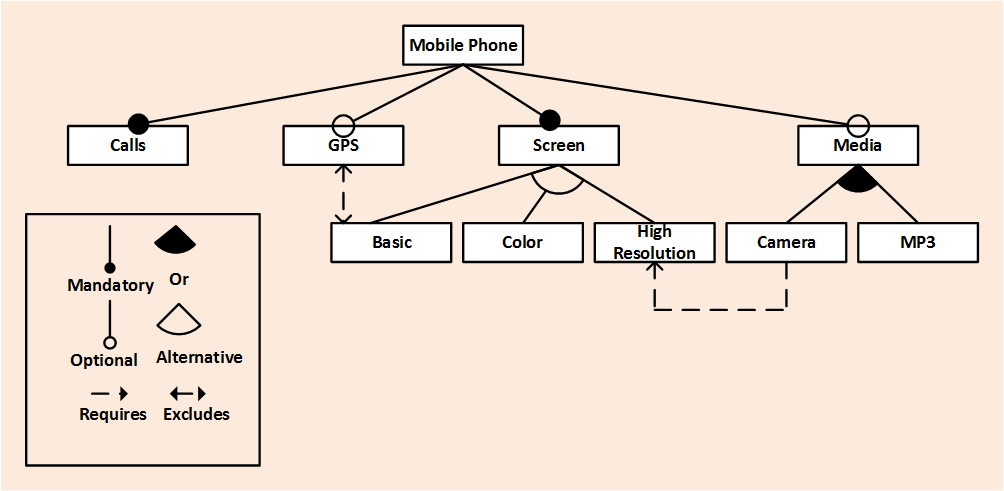
\includegraphics[width=\linewidth]{img/ft.png}
\caption{Feature model for mobile phone product line. To form a mobile phone, ``Calls'' and ``Screen'' are the mandatory features(shown as \textit{solid $\bullet$}), while the ``GPS'' and ``Media'' features are optimal(shown as \textit{hollow $\circ$}). The ``Screen'' feature can be ``Basic``, ``Color'' or ``High resolution'' (the \textit{alternative} relationship). The ``Media'' feature contains ``camera'', ``MP3'', or both (the \textit{Or} relationship).}
\label{fig:mobile}
\end{figure}


Figure \ref{fig:mobile} shows a feature model for a mobile phone
product line. All features are organized as a tree. The relationship
between two features might be ``mandatory'', ``optional'',
``alternative'', or ``or''. Also, there exist some cross-tree constraints, which means the preferred features are not in the same sub-tree. These cross-tree constraints complicate the process of exploring feature models\footnote{Without cross-tree constraints, one can generate products in linear time using a top-down traversal of the feature model.}. 
Researchers who explore these kinds of models~\cite{sayyad13a, sayyad13b, harman2014search, henard2015combining}
define a ``good'' product as the one that satisfies five objectives:
(1) find the valid products (products not violating any cross-tree constraint or tree structure), (2) with more features, (3) less known defects, (4) less total cost, and (5) most features used in prior applications.

\noindent\textbf{Challenges: } Finding a valid product in real-world software product lines can be very difficult due to the sheer scale of these product lines. Some software product line models comprise up to tens of thousands
of features,  with 100,000s of constraints. These constraints make it difficult to generate valid product through random assignments (similar to \textit{generate} function in Figure~\ref{fig:EA}). In some cases, chances of finding valid solutions through random assignment is $0.04\%$. Most of the meta-heuristic algorithms often fail to find valid solutions or take a long time to find one. Given the large and constrained search space ($2^N$, where N is the number of features) using an EA algorithm can be infeasible.

\noindent\textbf{Strategy:} Since exploring all the possible solutions is expensive and often infeasible. The SWAY, or the ``Sampling WAY'', cluster the individual products based on their features. Please note, clustering does not require evaluations---to find the fitness of each product. SWAY uses a domain-specific distance function to cluster the points. A domain-specific distance function was required because (1) clusters should have similar products---similar fitness values, and (2) the decision space is a boolean space. This is in line with the observation of Zhang et al.~\cite{zhang2013software}, who reports that MSR practitioners understand the data using domain knowledge. Once the products are clustered, a product is selected (at random) from each cluster. Based on the fitness values of the `representative product,' the not so promising clusters are eliminated. This step is similar to the \textit{elitism} operator of EAs. This process continues recursively till a certain budget is reached. Please refer to \cite{nair2016accidental, chen2017beyond, chen2017sampling} for more details. The reproduction package of SWAY and associated material can be found in \url{http://tiny.cc/raise_spl}.


\subsection{Performance Configuration Optimization}
\noindent\textbf{Problem Domain: } SBSE

\noindent\textbf{Problem: } Modern software systems come with a lot of knobs or configuration options, which can be tweaked to modify the functional or non-functional (e.g., throughput or runtime). Finding the best or optimal configuration to run a particular workload is essential since there is a significant difference between the best and the worst configurations. Many researchers report that modern software systems come with a daunting number of configuration options~\cite{xu2015hey}. The size of the configuration space increases exponentially with the number of configuration options. The long runtimes or cost required to run benchmarks make this problem more challenging.

\noindent\textbf{Challenges: } Most prior work in this area used a machine learning method to accurately model the
configuration space. The model is built sequentially, where new configurations are sampled randomly, and the quality
or accuracy of the model is measured using a holdout set. The size of the holdout set in some cases could be up to 20\% of the configuration space~\cite{nair2017using} and need to be evaluated (i.e., measured) before even the machine learning model is fully built. This strategy makes these methods not suitable in a practical setting since the generated holdout set can be (very) expensive. On the other hand, there are software systems for which an accurate model cannot be built. 

\noindent\textbf{Strategy: } The problem of finding the (near) optimal configuration is expensive and often infeasible using the current techniques. A useful strategy could be to build a machine learning model which can differentiate between the good and not so good solutions. Flash, a Sequential Model-based Optimization (SMBO), is a useful
strategy to find extremes of an unknown objective. Flash is
efficient because of its ability to incorporate prior belief as
already measured solutions (or configurations), to help direct
further sampling. Here, the prior represents the already
known areas of the search (or performance optimization) problem. The prior can be used to estimate the rest of the
points (or unevaluated configurations). Once we have evaluated
one (or many) points based on the prior, we can define
the posterior. The posterior captures our updated belief in
the objective function. This step is performed by using a
machine learning model, also called surrogate model. 
The concept of Flash can be simply stated as:
\begin{itemize}
\item Given what we know about the problem,
\item what should we do next?
\end{itemize}
The ``given what we know about the problem'' part is
achieved by using a machine learning model whereas ``what
should we do next'' is performed by an acquisition function.
Such acquisition function automatically adjusts the exploration
(``should we sample in uncertain parts of the search
space'') and exploitation (``should we stick to what is already
known'') behavior of the method. Please refer to  \cite{nair2018finding} and  \cite{nair2017using,nair2017faster} to similar strategies. The reproduction package is available in \url{http://tiny.cc/flashrepo/}.


\subsection{Topic Modelling}
\noindent\textbf{Problem Domain: } MSR

\noindent\textbf{Problem:} Currently a grand challenge in software analytics is understanding unstructured data. One of the ways is to provide a gist about this unstructured text into few related topics (an area called topic modeling), which can be done using Latent Dirichlet allocation (LDA). But what if these topics generated are misleading due to a systematic error found in LDA. This error exists in all kinds of non-deterministic and probabilistic-based method. Especially in the case of streaming data, your input order of data to LDA is changing which leads to different outputs~\cite{gennari1989models}. If these topics generated being used in an unsupervised task such as to make a conclusion or supervised task such as predicting for a text document to be relevant or not, your results could be wrong. A good topic model is the one in which topics generated are consistent, and effect of randomness due to input order has been effectively reduced.

\noindent\textbf{Challenges: } Researchers have found this kind of error/instability in the generated LDA topic model but have hardly done any work to reduce its effects. For this error to exist, it is essential that input order of data needs to be changed and this usually happens when LDA is run over a stream of data inputs. Once it is identified that the input order is changed, optimization of LDA can be done. But due to such a large space of configurations, finding an optimal configuration is an expensive task. 

\noindent\textbf{Strategy:} Exploring all possible configurations either using a Grid search or traditional EA is an expensive task. For this, we propose an intelligent search-based optimizer, called Differential Evolution (DE), which generates different configurable parameters by supporting vector level mutation. This new method, called LDADE, reduces the effects created due to order effects. The topics generated by LDADE are consistent and gave good performance for an unsupervised and supervised task. Please refer to~\cite{agrawalwrong} for more details. The reproduction package and associated material can be found at \url{https://github.com/ai-se/Pits_lda}.

 \subsection{Requirements Models}
    \textbf{Problem Domain: } SBSE
    
    \noindent\textbf{Problem:} Prior work ~\cite{Lamsweerde2001,amyot10} shows that the process of building and analyzing complex requirements engineering models can help stakeholders better understand the ramifications of their decisions. But models can sometimes overwhelm stakeholders. For example, consider a committee reviewing a goal model(see fig. \ref{fig:csServices}) that describes the information needs of a computer science department. Although the model is entangled, on manual and careful examination, we observe that much of the model depends on a few ``key'' decisions such that once their values are assigned, it becomes very simple to reason over the remaining decisions. It is beneficial to look for these ``keys'' in requirements models since, if they exist, we can achieve ``shorter'' reasoning about large RE models, where ``shorter'' is measured as follows:
    \begin{itemize}
     \item{Large models can be processed in a very short time.}
     \item{Runtimes for automatic reasoning about RE models are shorter so stakeholders can get faster feedback on their models.}
     \item{The time required for manual reasoning about models is shorter since stakeholders need only debate a small percent of the issues (just the key decisions).}
    \end{itemize}
   
    
    \begin{figure}[!t] 
  ~~~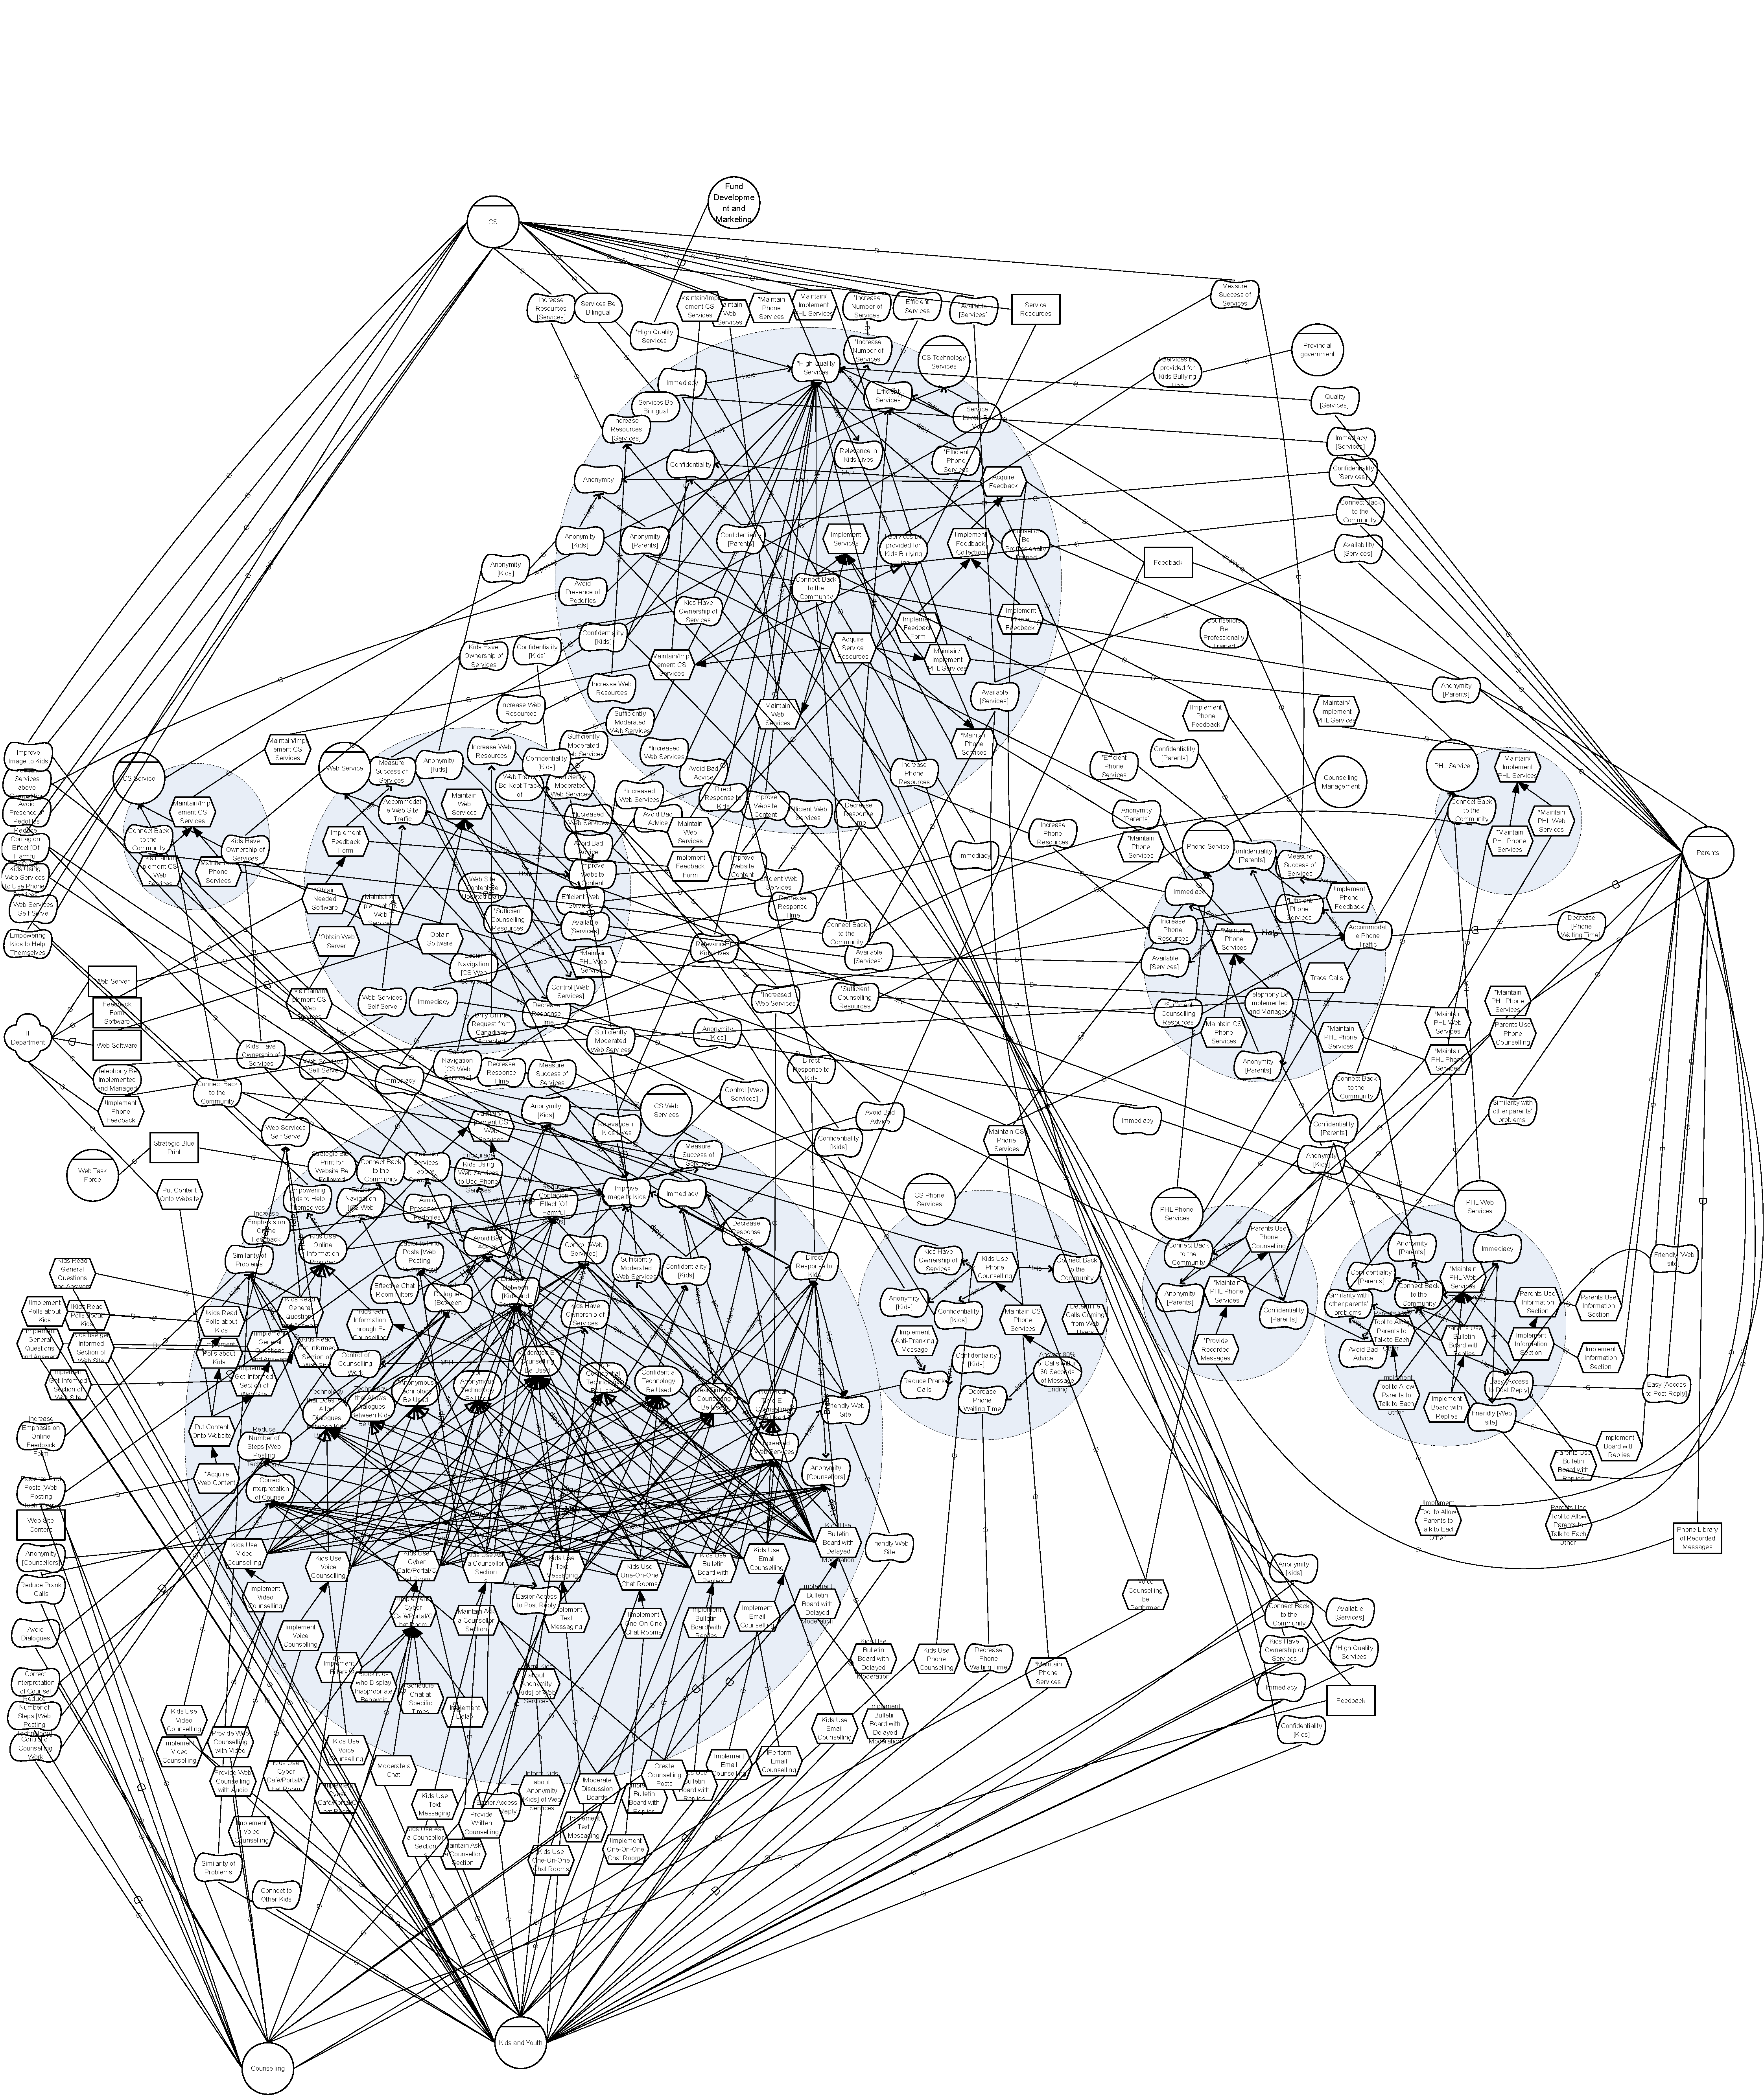
\includegraphics[width=3.1in]{img/CSServices.pdf} 
    \caption{Options for services in a CS department (i* format).}
    \label{fig:csServices}
\end{figure}


Such models are represented using the \textit{i*} framework \cite{yu97a} which include the key concepts of NFR~\cite{mylopoulos92.nfr} framework, including softgoals, AND/OR decompositions and contribution links along with goals, resources, and tasks. The i* framework describes dependencies among actors. There are four primary elements to describe the model: \textbf{goal}, \textbf{soft goal}, \textbf{task} and \textbf{resource}. Intentional actor forms the central concept in i*. Organizational actors are viewed as having intentional properties such as goals, beliefs, abilities, and commitments (a concept of distributed intentionality). Actors depend on each other for goals to be achieved, tasks to be performed and resources to be generated. By depending on others, an actor may be able to achieve goals that are difficult or impossible to achieve on its own. On the other hand, an actor becomes vulnerable if the actors it depended on did not deliver. Actors are strategic in the sense that they are concerned about opportunities and vulnerabilities and seek rearrangement of their environments that would better serve their interests by restructuring intentional relationships. 

\noindent\textbf{Challenges: } Committees have trouble with manually reasoning about all the conflicting relationships in models like fig. \ref{fig:csServices} due to its sheer size and numerous interactions(This model has 351 node, 510 edges and over 500 conflicting relationships). Further, automatic methods for reasoning about these models are hard to scale up: as discussed below, reasoning about inference over these models is an NP-hard task. 

\noindent\textbf{Strategy:} To overcome this problem, we propose a technique called SHORT which runs in four phases:
\begin{itemize}
    \item{\textbf{SH}: 'S'ample 'H'euristically the possible labelings of the model.}
    \item{\textbf{O}: 'O'ptimize the label assignments to cover more goals or reduce the sum of the cost of the decisions in the model.}
    \item{\textbf{R}: R: 'R'ank all decisions according to how well they performed during the optimization process.}
    \item{\textbf{T}: T: 'T'est how much conclusions are determined by the decisions that occur very early in that ranking.}
\end{itemize}

We used the above technique on eight large real-world Requirements Engineering models. We were able to that all of these models have under 25\% of their decisions as ``keys'' and 6 of them had less than 12\% decisions as keys. The process of identifying keys was also fast as it could run in near linear time with the largest of models running in less than 18 seconds. Please refer to \cite{mathew2017shorter} for more details and the reproduction package can be found at \url{http://tiny.cc/raise_short}.

\subsection{FASTREAD}
\noindent\textbf{Problem Domain: } SBSE

\noindent\textbf{Problem: }
Research in any field starts with learning about the field by reading the literature of that field (and sometimes attending lectures). The process of finding relevant papers to read is often challenging, and it is easy to miss out on important papers. Broad and complete literature reviews are required when (1) researchers are exploring a new area; (2) researchers writing papers for peer review, to ensure reviewers will not reject a paper since it omits important related work; and (3) anyone surveying a field for latest developments. This problem can also be generalized as following: How to maximize relevant information (when there is a lot of noise) while minimizing the search cost to find relevant information?
   
\vspace{1.0ex}
\noindent\textbf{Challenge 1: }
Literature reviews can be extremely labor intensive and often require months (if not year) to complete. Due to a large number of papers available, the relevant papers have hard to find. A graduate student needs to review thousands of papers before finding few dozen relevant papers. 

\noindent\textbf{Strategy: }
   Since, reading all the literature available in infeasible, we need to use an active learner. Such active learner incrementally learns from the human feedback and suggests on which paper to review next so that most relevant papers can be found by reviewing a minimal number of papers.
   
\vspace{1.0ex}
\noindent\textbf{Challenge 2: }
It is important to note that the initial papers chosen to be reviewed can dramatically reduce the variance in the review effort. A wrong choice of initial papers can increase the effort by up to 300\% than the median effort (repeat for 30 runs)---requires three times more effort to retrieve the relevant papers. 

\noindent\textbf{Strategy: }
Such variances can be alleviated by selecting a good initial set of papers with domain knowledge from the researcher. We found that by ranking the papers with their BM25 scores of a set of keywords (provided as domain knowledge) and reviewing in such order, the effort can be further reduced with negligible variances.
   
\vspace{1.0ex}
\noindent\textbf{Challenge 3: }
Another challenge is when to stop the reviewing process. Stopping too early will result in many missing relevant papers while stopping too late could waste review effort on irrelevant papers. The desired stopping point would be when 95\% of the relevant papers have been found. However, since we do not know the total number of relevant papers to be found, there is no way to know whether we have found 95\% of it.

\noindent\textbf{Strategy: }
Stopping criterion for most of the search algorithms is based on either resource constraints or a predefined stopping criterion (historical knowledge). However, this is not suitable for this problem setting. A possible way to determining the stopping criterion is to use a semi-supervised machine learning algorithm (Logistic Regression) learn from the search process (till now) to predict how much more relevant paper will be found.The predicted values from this regressor are used to decide when to stop the process of search.
   
\vspace{1.0ex}
\noindent\textbf{Challenge 4: }
Actual human reviewers are fallible when labeling the papers. Research shows that it is reasonable to assume the precision and recall of a human reviewer are both 70\%. When such human errors occur, how to correct the errors so that the active learner is not misled?

\noindent\textbf{Strategy: }
The intuition used to solve the problem is the following: concentrate the effort on correctly classifying the paper which creates the most controversy. Using this intuition, periodically few of the already evaluated papers, whose labels the active learner disagree most on, are re-evaluated.

\subsection{Text classification}
\noindent\textbf{Problem Domain: } MSR

\noindent\textbf{Problem: } Stack Overflow is a popular Q\&A website, where users posts the questions and the community collectively answers these questions. However, as the community evolves, there is chance that duplicate questions can appear---which results in a wasted effort of the community. There is a need to remove the duplicate question or consolidate related questions. The problem focuses on discovering the relationship between any two questions posted on Stack Overflow and classifies them into duplicates, direct link, indirect link, and isolated~\cite{fu2017easy, xu2016predicting}. One way to solve this problem is to build a predictive model which can predict the similarity between two questions. 

\noindent\textbf{Challenge: } The state of the art method for this problem used a Deep Learning method, which was expensive to train~\cite{xu2016predicting}. For example, Xu et al. spent 14 hours to train a deep learning model. Such long training time is not appropriate for the field of software analytics since software analytics requires the methods to have a fast turnaround time~\textcolor{red}{cite the paper which says fast turn around time is required}.

\noindent\textbf{Strategy: }To reduce the training time as well as promote simplicity, hyper-parameter optimization of simple learners, like SVM (Support Vector Machines), is a way to go. Specifically, a Differential Evolution algorithm, which has been an effective tuning algorithm (used in SBSE)~\cite{fu2016tuning},
to explore the parameter space of SVM. After the search process,
 SVM with best-found parameters is used to predict classes of Stack Overflow questions. This method can get similar or better results
than the deep learning method while reducing the training time by up to 80 times. Please refer to \cite{fu2017easy} for more details. Please refer to \cite{fu2017easy} for more details and the reproduction package can be found in~\url{http://tiny.cc/raise_data_easy}.

\begin{figure}[!b]
    \centering
    \noindent
    \begin{tabular}{cccccc}
        % Montage
        \resizebox{!}{70pt}{
        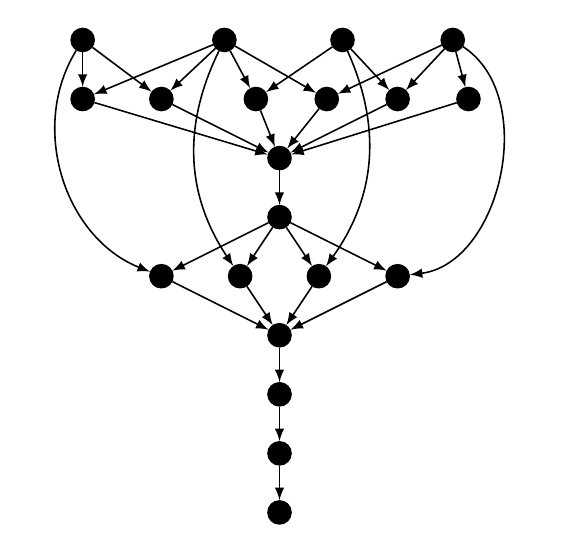
\begin{tikzpicture}
[lineDecorate/.style={-latex,line width=0.2mm}, nodeDecorate/.style={shape=circle,inner sep=3pt,draw}]

 \foreach \nodename/\x/\y in {
0/0/0,
1/1/0,
2/2/0,
3/3/0,
4/1.5/-0.5,
5/1.5/-1.0,
6/1.5/-1.5,
7/1.5/-2,
8/-1/2,
9/0.8/2,
10/2.3/2,
11/3.7/2,
12/-1/1.5,
13/0/1.5,
14/1.2/1.5,
15/2.1/1.5,
16/3/1.5,
17/3.9/1.5,
18/1.5/1.0,
19/1.5/0.5
 }
 {
          \node (T\nodename) at (\x,\y*1.5) [nodeDecorate, fill=black] {};
 }
		
\path
\foreach \startnode/\endnode in {0/4,1/4,2/4,3/4,4/5,5/6,6/7,
8/12,8/13,9/12,9/13,9/14,9/15,10/14,10/16,11/15,11/16,11/17,
12/18,13/18,14/18,15/18,16/18,17/18,
18/19,
19/0,19/1,19/2,19/3}
        {
          (T\startnode) edge[lineDecorate] node {} (T\endnode)
        }

(T8) edge[lineDecorate, bend right=50] node{} (T0)
(T10) edge[lineDecorate, bend left=30] node{} (T2)
(T9) edge[lineDecorate, bend right=30] node{} (T1)
(T11) edge[lineDecorate, bend left=70] node{} (T3);
        \end{tikzpicture}}
         
& 
% Epigenomics
\resizebox{!}{70pt}{
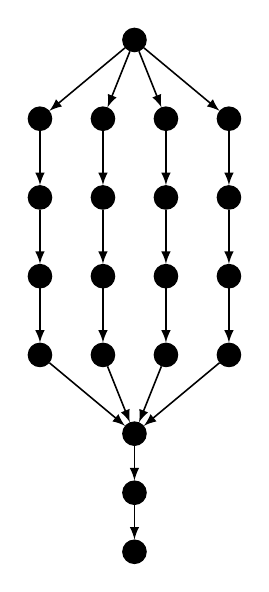
\begin{tikzpicture}
[lineDecorate/.style={-latex,line width=0.2mm}, nodeDecorate/.style={shape=circle,inner sep=3pt,draw}]

 \foreach \nodename/\x/\y in {
0/1.5/0,
1/1.5/-0.5,
2/1.5/-1
 }
 {
          \node (T\nodename) at (\x*0.8,\y*1.5) [nodeDecorate, fill=black] {};
 }
		
		
		 \foreach \x in {0,1,2,3}
 {
          \node (A\x) at (\x*0.8, 4.0) [nodeDecorate, fill=black] {};
		  \node (B\x) at (\x*0.8, 3.0) [nodeDecorate, fill=black] {};
		  \node (C\x) at (\x*0.8, 2.0) [nodeDecorate, fill=black] {};
		  \node (D\x) at (\x*0.8, 1.0) [nodeDecorate, fill=black] {};
 }
 
 \node(H) at (1.5*0.8, 5) [nodeDecorate, fill=black]{};
 
\path
\foreach \startnode/\endnode in {0/1,1/2}
        {
          (T\startnode) edge[lineDecorate] node {} (T\endnode)
        }
\foreach \startnode/\endnode in {H/A1,H/A2,H/A3,H/A0}
        {
          (\startnode) edge[lineDecorate] node {} (\endnode)
 }
 
 \foreach \i in {0,1,2,3}
        {
          (A\i) edge[lineDecorate] node {} (B\i)
		  (B\i) edge[lineDecorate] node {} (C\i)
		  (C\i) edge[lineDecorate] node {} (D\i)
		  (D\i) edge[lineDecorate] node {} (T0)
 };

        
\end{tikzpicture}}

% Inspiral
 \hspace{.2in}\resizebox{!}{70pt}{
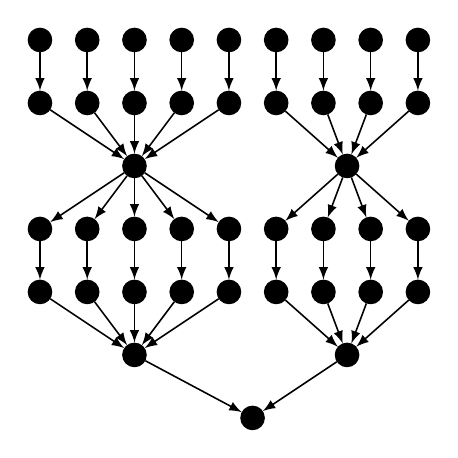
\begin{tikzpicture}
[lineDecorate/.style={-latex,line width=0.2mm}, nodeDecorate/.style={shape=circle,inner sep=3pt,draw}]

 \foreach \i in {0,1,2,3,4,5,6,7,8}
 {
          \node (A\i) at (\i*0.6,5*0.8) [nodeDecorate, fill=black] {};
		  \node (B\i) at (\i*0.6,4*0.8) [nodeDecorate, fill=black] {};
		  \node (E\i) at (\i*0.6,2*0.8) [nodeDecorate, fill=black] {};
		  \node (F\i) at (\i*0.6,1*0.8) [nodeDecorate, fill=black] {};
 }
 \node(C) at (2*0.6,3*0.8) [nodeDecorate, fill=black]{};
 \node(D) at (6.5*0.6,3*0.8) [nodeDecorate, fill=black]{};
 \node(G) at (2*0.6,0*0.8) [nodeDecorate, fill=black]{};
 \node(H) at (6.5*0.6,0*0.8) [nodeDecorate, fill=black]{};
  \node(I) at (4.5*0.6,-1*0.8) [nodeDecorate, fill=black]{};
\path

 \foreach \i in {0,1,2,3,4,5,6,7,8}
        {
          (A\i) edge[lineDecorate] node {} (B\i)
		  (E\i) edge[lineDecorate] node {} (F\i)
 }
  \foreach \i in {0,1,2,3,4}
        {
          (B\i) edge[lineDecorate] node {} (C)
		  (C) edge[lineDecorate] node {} (E\i)
		  (F\i) edge[lineDecorate] node {} (G)
 }
  \foreach \i in {5,6,7,8}
        {
          (B\i) edge[lineDecorate] node {} (D)
		  (D) edge[lineDecorate] node {} (E\i)
		  (F\i) edge[lineDecorate] node {} (H)
 }

 (G) edge[lineDecorate] node {} (I)
 (H) edge[lineDecorate] node {} (I);
\end{tikzpicture}}


\\
~\\

% CyberSkake
\resizebox{!}{50pt}{
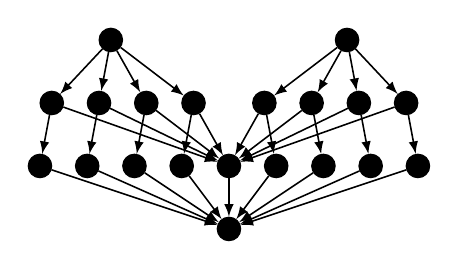
\begin{tikzpicture}
[lineDecorate/.style={-latex,line width=0.2mm}, nodeDecorate/.style={shape=circle,inner sep=3pt,draw}]

 \foreach \i in {0,1,2,3}
 {
          \node (A\i) at (\i*0.6+0.15,1*0.8) [nodeDecorate, fill=black] {};
		  \node (B\i) at (\i*0.6,0*0.8) [nodeDecorate, fill=black] {};
		  
 }
 
  \foreach \i in {5,6,7,8}
 {
          \node (A\i) at (\i*0.6-0.15,1*0.8) [nodeDecorate, fill=black] {};
		  \node (B\i) at (\i*0.6,0*0.8) [nodeDecorate, fill=black] {};
		  
 }
 
 \node(X) at (1.5*0.6, 2*0.8) [nodeDecorate, fill=black]{};
 \node(Y) at (6.5*0.6, 2*0.8) [nodeDecorate, fill=black]{};
\node(K) at (4*0.6, 0*0.8) [nodeDecorate, fill=black]{};
\node(E) at (4*0.6,-1*0.8) [nodeDecorate, fill=black]{};
\path

 \foreach \i in {0,1,2,3}
        {
          (A\i) edge[lineDecorate] node {} (B\i)
		  (A\i) edge[lineDecorate] node {} (K)
		  (B\i) edge[lineDecorate] node {} (E)
		  (X) edge[lineDecorate] node {} (A\i)
 }
 (K) edge[lineDecorate] node{}(E)
  \foreach \i in {5,6,7,8}
        {
          (A\i) edge[lineDecorate] node {} (B\i)
		  (A\i) edge[lineDecorate] node {} (K)
		  (Y) edge[lineDecorate] node {} (A\i)
		  (B\i) edge[lineDecorate] node {} (E)
 };
 
\end{tikzpicture}}


&

% Sipht
\resizebox{!}{50pt}{
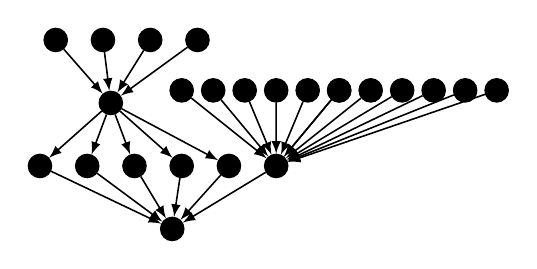
\begin{tikzpicture}
[lineDecorate/.style={-latex,line width=0.2mm}, nodeDecorate/.style={shape=circle,inner sep=3pt,draw}]

 \foreach \i in {0,1,2,3,4}
 {
          \node (A\i) at (\i*0.6,-1*0.8) [nodeDecorate, fill=black] {};
		  
 }
 
  \foreach \i in {0,1,2,3}
 {
          \node (C\i) at (\i*0.6+0.2,1*0.8) [nodeDecorate, fill=black] {};
		  
 }
 
   \foreach \i in {0,1,2,3,4,5,5,6,7,8,9,10}
 {
          \node (F\i) at (\i*0.4+1.8,0.2*0.8) [nodeDecorate, fill=black] {};
		  
 }
 
 \node(B) at (1.5*0.6, 0*0.8) [nodeDecorate, fill=black]{};
 \node(D) at (2.8*0.6, -2*0.8) [nodeDecorate, fill=black]{};
  \node(E) at (5*0.6, -1*0.8) [nodeDecorate, fill=black]{};
\path
(E) edge[lineDecorate] node {} (D)  
 \foreach \i in {0,1,2,3}
        {
          (C\i) edge[lineDecorate] node {} (B)  
 }
  \foreach \i in {0,1,2,3,4}
        {
          (A\i) edge[lineDecorate] node {} (D)
		  (B) edge[lineDecorate] node {} (A\i)
 }
   \foreach \i in {0,1,2,3,4,5,5,6,7,8,9,10}
        {
          (F\i) edge[lineDecorate] node {} (E)
 };
\end{tikzpicture}}



\\
    \end{tabular}
    \caption{
    Some  of  cloud computing  workflows. Clockwise from top left: {\tt Montage, Epigenomics, Inspiral, CyberShake, Sipht}. Each node is one ``task''
    and each edge is a data flow from one task to another.   Number of tasks  can vary from dozens to   thousands).  The configuration problem is to map these tasks to a smaller number
    of virtual machine instances, decide the ordering of tasks within one instance, and
    then decide what kind of machine should drive each instance. For description  of these workflows, see Table~\ref{tab:workflows}.
    }
    \label{fig:structure}
\end{figure}

\subsection{Workflows in Cloud Environment}
\textbf{Problem Domain: } SBSE


\noindent\textbf{Problem:} Many complex computational tasks, especially in a scientific area, can be divided into several sub-tasks where outputs of some tasks servers the input of another task. A workflow is a tool to
model such kind of computational tasks.



Figure \ref{fig:structure} shows five types of widely studied workflows. Workflows are represented as a directed acyclic graph (DAG). Each vertex of the DAGs represents one sub-task. Connections between vertices represent the result communications between different vertices. One computational task is called ``finished'' only when
all sub-tasks are finished. Also, all executions of sub-tasks should follow the constraints per edges.

Grid computing techniques, invented in the mid-1990s, as well as recently, lots of pay-as-you-go cloud computing services, e.g., Amazon EC2, provide researchers a feasible way to finish such kind of complex workflow in a reasonable time.
The workflow configuring problem is to figure out the best deployment configurations onto a cloud environment. The deployment configuration
contains 1) determine which sub-tasks can be deployment into
one computation node, i.e., the virtual machine in cloud environment; 2) which sub-task should be executed first if two of them are to be executed in the same node; 3) what hardware configuration (CPU, memory, bandwidth, etc.) should be applied in each computation node. Notice that commercial cloud service provider charges users for computing resource. 
The objective of cloud configuration is to minimize the monetary cost as well as minimize the runtime of computing tasks.


\noindent\textbf{Challenges: } 
Two reasons make workflow configuration on cloud environment challenging: 1)  a number of sub-tasks of workflows can be as large as hundreds, or thousands; also, sub-tasks is under constraints-- file flow between them. 2) available types of
computing nodes from cloud service provided is huge.
For example, Amazon AWS provides more than 50 types of virtual machines; these
virtual machines have different computing ability, as well as unit price (from \$0.02/hr to \$5/hr).
Given these two reasons,
the configuration space, or a number of possible deployment ways, is huge.
Even though modern cloud environment simulator, such as CloudSim, can quick
access performance of one deployment, evaluate every
possible deployment configuration is impossible.

\noindent\textbf{Strategy:} 
Since it is impossible to enumerate all possible configurations, most existed algorithm use either 1) greedy algorithm 2) evolutionary algorithm to figure out best configurations.
Similar to other search-based software engineering problems,
these methods require a large number of model evaluations (simulations in workflow configuration problem).
The RIOT, or randomized instance-order-type, is an algorithm to balance execution time as well as cost
in a short time.
The RIOT first groups sub-tasks, making the DAG simpler, and then
assign each group into one computation node. Within one node,
priorities of sub-tasks are determined by
B-rank~\cite{topcuoglu2002performance}, a greedy algorithm. 
The most tricky part is to determine types of computation nodes so that they can coordinate with each other and reduce the total ideal time (due to file transfer constraints).
In RIOT,
we make full use of two hypothesis: 1) similar configurations should have similar performance; 2) (monotonicity) k times computing resource should lead to (1/k)*c less computation time (where c is constant for one workflow).
With these two hypotheses,
RIOT first randomly creates some deployment configurations and evaluates them, then guess more configurations based on current evaluated configuration. Such kind of guess can avoid a large number of configuration evaluations. Please refer to \cite{chen2017riot} for more details and the reproduction package is available in \url{http://tiny.cc/raise_gen_workflow}.


\section{Conclusions}
Software engineering problems can be solved both by MSR and SBSE techniques, but both these methods have their shortcomings. This paper has argued these shortcomings can be overcome by merging ideas from both these domains, to give rise to a new field of software engineering called Data-Driven Search-based Software Engineering. This sub-area of software engineering boost the techniques used in MSR and SBSE but drawing inspiration from the other field. 

The paper proposes concrete strategies which can be used to combine the techniques from MSR and SBSE to solve an SE problem. The paper also lists resource which can be used researchers to jump-start their research. One of the aims of the paper is to provide resources and material which can be used as teaching or training resources for a new generation of researchers. 

% \bibliographystyle{ACM-Reference-Format}
% \bibliography{sample-bibliography}

\bibliographystyle{ACM-Reference-Format}
\bibliography{References} 

\end{document}
